
\chapter{The Mathematical Origins of Exploration}

\section{Introduction} 

In the previous chapter, we have seen the importance and benefits of \emph{information-seeking} as opposed to \emph{random} exploration for reinforcement learning tasks. Information-seeking exploration, which explicitly aims to reduce uncertainty about either the environment or the agent's model of the environment, provides a powerful exploration strategy that allows the rapid and efficient exploration of an environment, as opposed to the random walk strategy employed by random exploration. Moreover, when combined in a single loss function with a reward maximizing term, this combination results in \emph{goal-oriented exploration} where the agent is only driven to explore contingencies which are also likely to lead to high reward. We have seen that this goal-directed, or goal-oriented, exploration mechanism has performed well in model-based reinforcement learning tasks including sparse-reward environments which are challenging for standard reinforcement learning agents. Moreover, this kind of exploration is almost certainly necessary for biological organisms in more ecologically valid tasks, where rewards are often very sparse and environments are typically very large compared to those in mainstream reinforcement learning benchmarks.

In this chapter, we take a more abstract perspective, and study in depth the question of the \emph{mathematical origin and meaning} of such goal-directed exploration objectives which unite both reward seeking and information maximizing terms in a single objective. Specifically, we seek to understand whence they arise, and what the mathematical formulation which can give rise to them is. While for practical purposes and engineering applications it is often sufficient to glue different terms together in an ad-hoc way to construct an objective which gives rise to some desired behaviour, we wish to probe the deeper theory underlying such functionals which has so far remained mostly mysterious. It is the hope that by mathematically understanding the origin and nature of such objectives, as well as their properties, we can illuminate a swathe of current methods in reinforcement learning, cognitive sciences, decision theory, and behavioural economics, as well as deeply understanding how they interrelate to one another. Moreover, it seems likely, given the generally productive dialectic between theory and practice in all of these fields, that by contributing to the underlying theory of such objectives, we can ultimately contribute to the design of more powerful objectives and methods than are currently used in the literature.

To begin, we wish to deeply examine the origin and nature of the \emph{Expected Free Energy} (EFE) functional. The EFE is central to the theory of active inference, where it is proposed that all agents under the free energy principle, which must seek to minimize the long term path integral of their surprise must choose policies that minimize the EFE. The EFE has been widely used in almost all models in discrete-time active inference \citep{friston_active_2015,friston2017active,friston2018deep,friston2017process,da2020active} with the exception of the later development of the generalized free energy \citep{friston2015active,parr2017uncertainty,parr2017active}.%, with some even going to far as to claim that the EFE `solves the exploration-exploitation dilemma' \citep{friston2020sophisticated,friston2015active,da2020active}.
  Despite this ubiquitous use within the active inference community, the precise mathematical origin and nature of the EFE functional have remained unclear. In the literature, the EFE is often justified through a \emph{reductio-ad-absurdum} argument \citep{friston2015active} which runs as follows -- since (we assume under the FEP) all agents minimize free energy, then they must think they will minimize free energy in the future. Since the future is uncertain, instead of the standard variational free energy (VFE), they must instead minimize their \emph{expected} free energy (EFE), else they are not a free-energy minimizing agent (disproven conclusion) \footnote{Technically this is more of an induction argument than a reductio-ad-absurdum, but we still refer to it as such due to its description as a reductio in the literature \citep{friston2015active}}. Central to this logic is the claim that the EFE is the `natural' extension of the VFE to account for uncertain futures. 

In the first section of this chapter, we investigate this claim in detail. Specifically, we argue that the EFE is not necessarily the only way to extend the VFE into the future, and that there are in fact other, more straightforward extensions, such as an objective we call the free energy of the future (FEF). We then perform a direct side-by-side comparison of the EFE and FEF functionals and comment on their similarities and differences, and discuss their respective bounding behaviour on the expected free energy. We then discuss how active inference approaches are related to the control as infrerence framework, and decide upon two key differences -- the objective functional utilized for action selection, where active inference uses the EFE, and control as inference uses the FEF, and secondly the encoding of value or goals into the inference process, where active inference directly encodes values into the generative model through the use of a biased desire distribution $\tilde{p}(o)$, control as inference instead uses independent optimality variables $p(\Omega | o)$ \footnote{We also denote any distribution involving a desire distribution with a $\tilde{p}$ and, for instance, refer to $\tilde{p}(o,x)$ as a \emph{biased generative model})}. Finally, we then introduce a second objective functional, which we call the free energy of the Expected Future (FEEF) which combines both an intuitively grounded starting point with the same exploration seeking term as is present in the EFE, and which was investigated previously in Chapter 4. We discuss the nature of different possible objective functionals for control.

In the second half of this chapter, we retreat from the specifics of the EFE, active inference, and control as inference, to instead define a general framework for understanding the origin of information seeking exploration terms in control functionals. We argue that the key distinction, is that between evidence objectives, which maximize the likelihood of achieving a desire distribution, with divergence functionals which try to minimize the divergence between a predicted and desire functional. Specifically, divergence objectives give rise to information gain terms while evidence objectives do not. We trace this capacity to the fact that divergence objectives implicitly maximize the entropy of the agent's future, in a close connection to empowerment objectives, while evidence objectives do not. Finally, we put all this together into a coherent framework which can be used to understand the full landscape of variational objective functionals for control tasks.

The material in this chapter is heavily based on three first-author papers. \emph{Whence the expected free energy} \citep{millidge2020whence} (published in neural computation), \emph{On the relationship between active inference and control as inference} (published at the IEEE international workshop on active inference) \citep{millidge2020relationship}, and \citep{millidge2021understanding} \emph{Understanding the Origin of Information-Seeking Exploration in Probabilistic Objectives for Control}, \emph{Arxiv} (to be submitted to Royal Society Interface).

\section{Origins of the Expected Free Energy}

Here we investigate the origins of the expected free energy (EFE) term within active inference. It is often claimed that the reason active inference agents minimize this term is that free energy minimizing agents must minimize the variational free energy (VFE) into the future which, since the future is uncertain, constitutes the \emph{expected} free energy. To make this claim precise, we need to understand exactly the variational free energy `into the future' should consist of. We argue that it must satisfy two conditions, which are both satisfied by the variational free energy, and which are crucial for that objective functions to operate. First, we argue that, like the VFE, the VFE extended into the future should be a divergence between a variational approximate posterior and a generative model of future states. Secondly, we argue that, again like the VFE, any free energy of the future should additionally be a bound on the log model evidence of future observations. These conditions are both important precisely because they define why the variational free energy is useful. Minimizing the divergence between the posterior and the generative model is useful since it implicitly makes the variational posterior a good approximation. Conversely, bounding the log model evidence is useful since the log-model evidence provides a very general measure of how `good' a specific model is, which can be used for Bayesian model-comparison or even just to understand the amount of inherent information in the data. Moreover, the log model evidence has especial import for methods under the aegis of the free energy principle since the log model evidence is simply the surprisal $-\ln p(o)$ which is the basic quantity which is minimized throughout the theory.

First, we need to define precisely the mathematical setup of the problem. We assume that our agent exists in a POMDP environment with states $x$, observations $o$, policies (sequences of actions) $\pi = [a_1, a_2 \dots a_T]$. The agent maintains a variational distribution over the states and actions and a generative model over the states, observations, and policies. Specifically, although we are technically interested in the functionals over a full trajectory $o_{1:T}$, in practice the functional decomposes into a sum of independent functionals for each timestep. Thus, for understanding the behaviour of agents optimizing the functional, it suffices to consider only a single timestep of the functional at $o_t$.

We argue that the expected free energy does not fulfil these conditions, but rather another objective functional does, which we call the free energy of the future (FEF). We define the FEF to be,
\begin{align*}
\mathbb{FEF}_t(\pi) &=  \mathbb{E}_{q(o_t, x_t | \pi)}[\ln q(x_t | o_t) - \ln \tilde{p}(o_t,x_t)] \\
&= \mathbb{E}_{q(o_t)}\KL[q(x_t | o_t) || \tilde{p}(o_t, x_t)] \numberthis
\end{align*}

which is simply the KL divergence between the approximate posterior generative model over future states, averaged under the expected future observations $q(o_t)$. This trivially satisifes the first condition, since it is a KL divergence between the variational posterior, and the generative model, as is the VFE. Next, we show that this functional is a bound on the expected log model evidence in the future.

\begin{align*}
    \label{FEF_bound}
    \numberthis
    - \mathbb{E}_{q(o_t | \pi)}\big[ \ln \tilde{p}(o_t) \big] &= - \mathbb{E}_{q(o_t | \pi)}\big[ \ln \int dx_t \tilde{p}(o_t,x_t) \big] \\
    &= - \mathbb{E}_{q(o_t | \pi)}\big[ \ln \int dx_t \tilde{p}(o_t,x_t) \frac{q(x_t | o_t)}{q(x_t | o_t)} \big] \\
    &\leq - \mathbb{E}_{q(o_t | \pi)}\int dx_t q(x_t | o_t) \big[ \ln  \frac{\tilde{p}(o_t,x_t)}{q(x_t | o_t)} \big] \\
    &\leq - \mathbb{E}_{q(o_t,x_t | \pi)} \big[ \ln  \frac{\tilde{p}(o_t,x_t)}{q(x_t | o_t)} \big] \\
    &\leq \mathbb{E}_{q(o_t,x_t | \pi)} \big[ \ln  \frac{q(x_t | o_t)}{\tilde{p}(o_t,x_t)} \big] \\
    &\leq \mathbb{E}_{q(o_t | \pi)}\mathbb{D}_{KL}[q(x | o_t)||\tilde{p}(o_t,x_t | \pi)] = \mathbb{FEF}(\pi) \numberthis
\end{align*}

Crucially, we can see that this is an \emph{upper bound} on the log model evidence, and thus minimizing the FEF will tend to decrease the gap between the FEF and the expected log-model evidence. This functional thus exhibits identical behaviour to the VFE. To gain a better understanding of the key differences between the EFE and the FEF, we can exhibit them side by side.

\begin{align*}
    \mathbb{FEF} &= \mathbb{E}_{q(o_t,x_t | \pi)}[\ln q(x_t | o_t) - \ln \tilde{p}(o_t,x_t)] \\
    \mathbb{EFE} &= \mathbb{E}_{q(o_t,x_t | \pi)}[\ln q(x_t | \pi) - \ln \tilde{p}(o_t,x_t)] \numberthis
\end{align*}

While the two formulations may look very similar, the key distinction is that the FEF optimizes the divergence between the variational \emph{posterior} $q(x_t | o_t)$ and the generative model while the EFE minimizes the variational \emph{prior} $q(x_t)$. While this difference may seem small, we see that it has a significant impact when it comes to the resulting interpretable terms from the decomposition of the two functionals,

\begin{align*}
    \label{FEFEFEComparison}
    \mathbb{FEF} &= -\underbrace{\mathbb{E}_{q(o_t,x_t | \pi)} \big[ \ln \tilde{p}(o_t | x_t) \big]}_{\text{Extrinsic Value}} + \underbrace{\mathbb{E}_{q(o_t | \pi)}\mathbb{D}_{KL}[q(x_t | o_t)||q(x_t | \pi)]}_{\text{Epistemic Value}} \numberthis \\
    \mathbb{EFE} &= \underbrace{-\mathbb{E}_{q(o_t,x_t | \pi)}\big[ \ln \tilde{p}(o_t) \big]}_{\text{Extrinsic Value}} -  \underbrace{\mathbb{E}_{q(o_t | \pi)}\mathbb{D}_{KL}[q(x_t | o_t)||q(x_t | \pi)]}_{\text{Epistemic Value}} \numberthis
\end{align*}

Specifically, we see that while both the FEF and the EFE can be split into `extrinsic' and `intrinsic' value terms, the intrinsic value term in the FEF is positive while in the EFE it is negative. Specifically this means that the FEF tries to \emph{minimize} exploration and keep the posterior and prior as close together as possible. This minimizing information gain term is analogous to the complexity term in the VFE which functions as a regulariser which attempts to keep the posterior as close to the prior as possible, while still fitting the data. Here, we see that the goal of the FEF is to, in effect, maximize reward, while trying to learn as little about the environment as possible. While this may seem to be an unfortunate objective, in some small cases it may be beneficial, especially when in the case of offline reinforcement learning, where there is no continual interaction with an environment, only trying to learn an optimal policy from a given dataset of interactions (\citep{levine2018reinforcement}. In such cases, failures of generalization and extrapolation can often result in poor results whenever the learned policy is moved even slightly off the data manifold, and this kind of conservative regularisation of the learning process can prove highly beneficial \citep{levine2020offline}. By contrast, the EFE \emph{maximizes} the information gain term, since it is negative, and tries to drive the posterior and prior as far apart as possible. This results in information-seeking exploration. 

However, while the EFE has an intuitively better exploratory grounding, it is not a bound on the log model evidence, as the FEF is. We can show this straightforwardly by noting that the `extrinsic value' term of the EFE simply \emph{is} the log model evidence,
\begin{align*}
    \mathbb{EFE} &= \mathbb{E}_{q(o_t,x_t | \pi)} [\ln q(x_t | \pi) - \ln \tilde{p}(o_t,x_t)] \\
    &\approx \mathbb{E}_{q(o_t,x_t | \pi)} [\ln q(x_t | \pi) - \ln q(x_t |o_t) - \ln \tilde{p}(o_t)] \\
    &\approx \underbrace{-\mathbb{E}_{q(o_t | \pi)} [ \ln \tilde{p}(o_t)]}_{\text{Negative Expected Log Model Evidence}} -  \underbrace{\mathbb{E}_{q(o_t | \pi)}\mathbb{D}_{KL}[ q(x_t | o_t) \Vert q(x_t | \pi)]|}_{\text{Information Gain}} \numberthis
\end{align*}
and that thus by the non-negativity of KL divergences, the EFE is a \emph{lower bound} on the log model evidence. This bound is in the wrong direction, since to make it tight, the EFE should be \emph{maximized} instead of minimized.

Importantly, in the definition of the EFE there is an approximation step where we have approximated $p(x_t | o_t)$ with the approximate posterior $q(x_t | o_t)$. If we make this approximation explicit, we can write the EFE as,

\begin{align*}
    \mathbb{EFE} &= \mathbb{E}_{q(o_t,x_t | \pi)} [\ln q(x_t | \pi) - \ln \tilde{p}(o_t,x_t)] \\
    &\approx \mathbb{E}_{q(o_t,x_t | \pi)} [\ln q(x_t | \pi) - \ln p(x_t |o_t) - \ln \tilde{p}(o_t)] \\
    &\approx \mathbb{E}_{q(o_t,x_t | \pi)} [\ln q(x_t | \pi) - \ln p(x_t |o_t) - \ln \tilde{p}(o_t) +\ln q(x_t |o_t) - \ln q(x_t | o_t)] \\
    &\approx \underbrace{\underbrace{-\mathbb{E}_{q(o_t | \pi)} [ \ln \tilde{p}(o_t)]}_{\text{Negative Expected Log Model Evidence}} +  \underbrace{\mathbb{E}_{q(o_t | \pi)}\mathbb{D}_{KL}[ q(x_t | o_t) \Vert p(x_t|o_t)]|}_{\text{Posterior Approximation Error}}}_{\text{FEF}}  \\ &-  \underbrace{\mathbb{E}_{q(o_t | \pi)}\mathbb{D}_{KL}[ q(x_t | o_t) \Vert q(x_t | \pi)]|}_{\text{Information Gain}} \numberthis
\end{align*}

Where we see that the EFE can be both an upper and lower bound on the log model evidence depending on whether the information  gain term or the posterior divergence term is larger. We can thus see that the likely time-course of the EFE is to cycle around the bound over the course of inference until, potentially, it reaches it. This is because, at the start of training, when inference is poor, the posterior divergence is likely greater than the information gain, so the EFE functions as an upper bound and minimizing it gets us closer to the true log model evidence. This effect likely quickly fades away as the information gain term becomes bigger, and here the EFE minimizing agent will preferentially explore its environment in an information-seeking fashion, driving the EFE \emph{away} from the real log model evidence for the environment. Finally, if there are no residual sources either of posterior divergence (so that the true and approximate posteriors are in the same class), or information gain (so that the agent has a perfect model of the environment, and the environment has no intrinsic stochasticity which gives rise to aleatoric uncertainty), then both the posterior divergence and the information gain terms will be 0, and the EFE will finally converge to exactly the log model evidence. While this behaviour of the EFE functional may lead to adaptive behaviour, it is not particularly mathematically principled as an extension to the VFE, and thus it is not necessarily clear why the EFE should be considered to be a better extension of the VFE than the FEF.

This derivation also reveals an interesting connection between the EFE and the FEF. Specifically, it is revealed that the EFE is simply the FEF minus an additional information gain term, thus effectively comprising the free energy into the future (FEF), with an additional exploratory information gain term. This derivation can also be derived straightforwardly from a direct comparison of the two functionals,

\begin{align*}
    \mathbb{FEF}_t(\pi) - \mathbb{IG}_t &= \mathbb{E}_{q(o_t,x_t | \pi)}\ln(\frac{q(x_t | o_t)}{\tilde{p}(o_t,x_t)}) - \mathbb{E}_{q(o_t,x_t | \pi)}\ln(\frac{q(x_t | o_t)}{q(x_t | \pi)}) \\
    &=  \mathbb{E}_{q(o_t,x_t | \pi)}\ln(\frac{q(x_t|o_t)q(x_t | \pi)}{\tilde{p}(o_t,x_t)q(x_t|o_t)}) \\ 
    &=  \mathbb{E}_{q(o_t,x_t | \pi)}\ln(\frac{q(x_t | \pi)}{\tilde{p}(o_t,x_t)}) \\
    &= \mathbb{EFE}(\pi)_t \numberthis
\end{align*}

We can thus understand the origin of the information gain term in the EFE -- it is simply the FEF into the future minus the information gain exploration term. This means that, in effect, the  exploratory properties of the EFE are simply present by construction. Is it possible, then, to derive mathematically or intuitively principled objectives which maintain the information seeking properties of the EFE?

While this question is definitively answered later in this chapter, here we present a hint of the solution. We propose a novel objective, which we call the free energy of the expected future (FEEF), which can be characterised simply as the divergence between the expected beliefs about future observations and states $q(o_t, x_t)$ and the desired distribution $\tilde{p}(o_t, x_t)$. The FEEF objective can be written as,

\begin{align*}
    \pi^* = \underset{\pi}{\mathrm{arg min}} \, \, \mathbb{D}_{KL}[q(o_{t:T},x_{t:T}|\pi)||\tilde{p}(o_{t:T},x_{t:T})] \numberthis
\end{align*}

In effect, this objective can be understood as compelling an agent to bring a predicted (variational) world and a desired (generative) distribution into alignment. This objective has a strong intuitive basis for understanding adaptive action, since we are simply trying to minimize the difference between our veridical beliefs about the future and our desires. Since the desire distribution is assumed fixed, the only way to maximize their alignment is to take action to force the predicted belief distribution towards the desired distribution. If the belief distribution is accurate, then this will result in trajectories that really do take the agent towards its desired distribution. Crucially, we can then decompose this objective into an extrinsic and intrinsic information seeking term, just like the EFE.
\begin{align*}
    \mathbb{FEEF}(\pi)_t &= \mathbb{E}_{q(o_t,x_t|\pi)} \ln \big[ \frac{ q(o_t,x_t |\pi)}{\tilde{p}(o_t,x_t )} \big] \\
    &\approx \underbrace{\mathbb{E}_{q(x_t | \pi)} \mathbb{D}_{KL} \big[ q(o_t | x_t) \Vert \tilde{p}(o_t) \big]}_{\text{Extrinsic Value}} - \underbrace{\mathbb{E}_{q(o_t | \pi)} \mathbb{D}_{KL} \big[ q(x_t | o_t) \Vert q(x_t | \pi) \big]}_{\text{Intrinsic Value}} \numberthis
\end{align*}

Here, we see that the epistemic information seeking term is identical to that of the EFE, and thus we would expect FEEF and EFE minimizing agents to show similar exploratory behaviour. The key difference between these objectives lies in the extrinsic value term. While the EFE simply aims to maximize the likelihood of the desire distribution under the variational belief distribution, the FEEF explicitly tries to minimize the KL divergence between them, and thus try to match the two distributions.

Another way of looking at the same thing is to consider this straightforward relationship between the EFE and the FEEF,
\begin{align*}
    \mathbb{FEEF}(\pi)_t &= \mathbb{D}_{KL} \big[ q(o_t, x_t) \Vert \tilde{p}(o_t,x_t) \big] \\
    &= \underbrace{\mathbb{E}_{q(o_t, x_t)}\big[ \ln q(o_t | x_t)]}_{\text{Observation Likelihood}} + \underbrace{\mathbb{E}_{q(o_t, x_t)}\big[ \ln \tilde{p}(o_t | x_t)] - \mathbb{E}_{q(o_t | \pi)} \mathbb{D}_{KL} \big[ q(x_t | o_t) \Vert q(x_t | \pi) \big]}_{\text{EFE}} \numberthis
\end{align*}

We can thus see, that the FEEF is simply the EFE plus an observation likelihood entropy term. This term is to be maximized and thus effectively provides an additional source of random exploration to the FEEF agent rather than the EFE. In effect, the FEEF agent optimizes the EFE while trying to keep its observation mapping as random as possible. Another advantage of the FEEF, is that it is equivalent to the VFE at the present time. This is because the observation entropy term is constant since it cannot be affected by future observations, and thus the expression as a whole reduces to the VFE. This means that the FEEF can be used as a unified objective for both perception and action, while the EFE can only be used for control. Due to this, a FEEF agent can have all distributions trained jointly on the FEEF objective while for an active inference agent, typically, if the transition and likelihood matrices are learnt, they are optimized against the VFE, while only action selection takes place using the EFE. This adds an additional degree of simplicity and elegance to FEEF-minimzing agents while they retain the same exploratory behaviours as active inference agents.

\subsection{Control as Inference and Active Inference}

This relationship between the FEF and the EFE sheds light upon the relationship between active inference and control as inference approaches to control. While the formulations at an abstract level are very similar -- both attempt to solve the control problem by deriving inference algorithms which operate on graphical models, and usually utilize the machinery of variational inference to do so -- at a lower detailed level the theories appear quite different and are presented with substantially differing motivations and notation. Using our newfound understanding of variational objective functionals of the future, such as the EFE and the FEF, here we pin down what exactly the relationship between control as inference and active inference is. 

First, we note that there are many straightforward notational differences between the theories which can be overcome. One obvious difference is that active inference is primarily concerned with the inferring of policies (or action sequences) while control as inference concerns itself with simply inferring policies, or single actions for a given timestep. It is important to note, however, that it is possible to reformulate active inference so that it infers policies, and, conversely, to reformulate control as inference so that it infers full action plans.  A second distinction is that active inference is typically formulated for POMDPs while control as inference only for MDPs. It is straightforward, however, to extend control as inference to the POMDP setup, which results in the following objective,
\begin{align*}
    \mathcal{L}(\phi)_{CAI} &= \KL \Big(q_\phi(x_t, a_t) \Vert p(x_t, a_t,o_t,\Omega_t) \Big) \\
    &= \underbrace{-\mathbb{E}_{q_\phi(x_t, a_t)}\big[ \ln p(\Omega_ | x_t, a_t) \big]}_{\text{Extrinsic Value}} + \underbrace{\KL \Big( q(x_t) \Vert p(x_t | x_{t-1},a_{t-1}) \Big)}_{\text{State divergence}} \\
    & \ \ + \underbrace{\mathbb{E}_{q(x_t)} \big[\KL \Big( q_\phi(a_t | x_t) \Vert p(a_t | x_t) \Big) \big]}_{\text{Action Divergence}} - \underbrace{\mathbb{E}_{q_\phi(x_t, a_t)}\big[ \ln p(o_t | x_t)\big]}_{\text{Observation Ambiguity}} \numberthis
\end{align*}
Here we have used notation standard in control as inference derivations, namely $q_\phi(a_t | x_t)$ is an amortized state-action policy and $\Omega_t$ is the `optimality variable'.
Importantly, this novel extension of control-as-inference to a POMDP setting leads directly to a straightforward implementation in terms of deep reinforcement learning, similar to the approaches in Chapter 4. Specifically, this objective can either be expressed directly as a sum over trajectories, and thus optimized by planning algorithms using model-based deep reinforcement learning or, alternatively, it can be expressed recursively and computed using a value or Q function approach which lends itself naturally to model-free deep reinforcement learning approaches. The key extension would be learning a probabilistic encoder-decoder model, most likely a VAE, to infer the distributions $q(x_t | o_t)$ and $p(o_t | x_t)$ and then to optimize the entropy of the VAE decoder in the control objective, in accordance with this objective function. Empirically investigating the performance of this method, and the impact of the observation ambiguity term, has not, to my knowledge, been explored in the literature, and would be an interesting avenue for further work. 

Secondly, we can similarly reformulate the control as inference approach to infer plans instead of policies. This is done by extending the generative model to cover whole trajectories instead of single observations, states, or actions. We then infer a constant random variable $\pi$ the policy for the whole trajectory. Written out explicitly, from this generative model you can derive a variant of the active inference optimal plan derivation to discover that the optimal plan under the control as inference is simply the softmax path integral over the variational free energy (VFE), augmented with optimality variables, and extended into the future.

\begin{align*}
    \mathcal{L}_{CAI} &= \KL \Big( q(x_{t:T}, \pi) \Vert p(x_{t:T}, \pi, o_{t:T}, \Omega_{t:T}) \Big) \\
    &= \KL \Big(q(\pi) \prod_t^T q(x_t | \pi) \Vert p(\pi) \prod_{t}^T p(\Omega_t | x_t, \pi)p(o_t | x_t)p(x_t | x_{t-1}, \pi) \Big)\\
    &= \KL \Big( q(\pi) \sum_t^T \KL \big[ q(x_t | \pi) \Vert p(\Omega_t | x_t, \pi)p(o_t | x_t)p(x_t | x_{t-1}, \pi) \big]\Vert p(\pi) \Big) \\
    &= \KL \Big( q(\pi)\Vert p(\pi) \exp(- \sum_t^T \mathcal{L}_t(\pi) ) \Big) 
    \implies q^*(\pi) = \sigma \Big(p(\pi) - \sum_t^T \mathcal{L}_t(\pi)\Big)  \numberthis
\end{align*}
We can decompose this VFE functional into the future as, 

\begin{align*}
    \mathcal{L}_t(\pi)_{CAI} &= \mathbb{E}_{q(x_t | \pi)}\big[ \ln q(x_t|\pi) - \ln p(x_t, \pi, o_t, \Omega_t)] \\
    &= -\underbrace{\mathbb{E}_{q(x_t | \pi)}\big[ \ln p(\Omega_t | x_t, \pi) \big]}_{\text{Extrinsic Value}} + \underbrace{\KL \Big(q(x_t | \pi) \Vert p(x_t | x_{t-1}, \pi) \Big)}_{\text{State divergence}} 
     - \underbrace{\mathbb{E}_{q(x_t | \pi)}\big[ \ln p(o_t | x_t) \big]}_{\text{Observation Ambiguity}}  \numberthis
\end{align*}

Which we can see is equivalent to the standard control as inference POMDP objective, except that it is missing the action divergence terms. The action divergence terms are missing simply because full policies are inferred instead of individual actions. Conversely, we can rederive active inference to infer individual actions rather than full policies. To do so, we simply need to add individual actions into the generative model and variational density and then crank through the derivation,

\begin{align*}
    -\mathcal{F}_t(\phi) &= \mathbb{E}_{q(o_t,x_t,a_t)}\Big[\ln q_\phi(a_t, x_t) - \ln \tilde{p}(x_t, o_t, a_t) \Big] \\
    &= -\underbrace{\mathbb{E}_{q(o_t|a_t)}\big[\ln \tilde{p}(o_t|a_t) \big]}_{\text{Extrinsic Value}} - \underbrace{\mathbb{E}_{q(o_t,a_t  | x_t)}\Big[ \KL \big( q(x_t | o_t, a_t) \Vert q(x_t|a_t) \big) \Big]}_{\text{Intrinsic Value}}  \\ &+ \underbrace{\mathbb{E}_{q(x_t)}\Big[ \KL \big( q_\phi(a_t | x_t) \Vert p(a_t | x_t) \big) \Big]}_{\text{Action Divergence}} \numberthis
\end{align*}
Here we see that the expression to be optimized with respect to the policy parameters $\phi$ is simply the standard active inference objective with an additional action-divergence term. If we assume the action prior $p(a_t | x_t)$ is uniform, then we regain the well known control as inference policy entropy term. Now that we have extended the theories to allow for a direct side-by-side comparison, we can see that the two major differences lie in the information gain term for active inference as opposed to the complexity `state-divergence' term for control as inference, and secondly that the control as inference approach contains an additional `likelihood entropy' term in its objective which active inference lacks. We know now that the information gain term in active inference arises directly from the definition of the EFE functional, which is not an intrinsic part of active inference and may not be theoretically justified. Indeed, if we replace the EFE in the active inference derivation with the FEF, we can obtain an objective identical to the control as inference approach except that it has no likelihood entropy term.

\begin{align*}
    -\hat{\mathcal{F}_t}(\phi) &= \mathbb{E}_{q_\phi(x_t, o_t, a_t)}\big[\ln q_\phi(x_t, a_t) - \ln \tilde{p}(o_t, x_t, a_t) \big]  \\
    &=  \underbrace{-\mathbb{E}_{q_\phi(x_t, a_t)}\big[ \ln \tilde{p}(o_t | x_t) \big]}_{\text{Extrinsic Value}} + \underbrace{\KL \Big( q(x_t) \Vert p(x_t | x_{t-1},a_{t-1}) \Big)}_{\text{State divergence}}  + \underbrace{\KL \Big( q_\phi(a_t | x_t) \Vert p(a_t | x_t) \Big)}_{\text{Action Divergence}} \numberthis
\end{align*}

This means that, effectively, we can consider control as inference as active inference with a FEF objective or, conversely, that active inference is simply control as inference with a nonstandard EFE objective. The question then remains, why does the control as inference objective possess an additional likelihood entropy term which active inference does not, since it is not due to a difference in objective function. We demonstrate that the difference actually arises due to the way goals or likelihoods are encoded in the inference procedure. Specifically, active inference encodes goals or rewards \emph{directly} into the generative model, so that active inference agents function with a biased generative model which blends reward-driven and veridical perception. By contrast, control as inference, keeps veridical inference and reward computation entirely separate, and instead includes rewards into the inference procedure through the use of exogenous optimality variables. The two methods thus solve subtly different inference problems due to these distinctions in how they encode rewards. Put simply, active inference encodes rewards and goals through priors; control as inference encodes them through conditioning.  Phrased intuitively, we can think of control as inference as solving the inference problem: \emph{Assuming that I have acted optimally in the future, what actions do I infer I will have taken}, while active inference solves the inference problem: \emph{Infer my most likely actions, given that I strongly believe in the future I will observe highly desirable states}. In sum, control as inference maintains a strict distinction between a veridical perceptual generative model, which generates objectively likely future outcomes for a given action sequence, while active inference maintains a biased generative model which preferentially predicts desired outcomes. Control as inference conditions this accurate generative model on observing high reward contingencies, and thus maintains an adaptive action plan. Active inference, on the other hand, simply maximizes the likelihood of this biased generative model, thus also inferring adaptive actions.

While this distinction may seem arcane, it actually speaks to deep philosophical differences in perspectives between the two theories. Control as inference arises from the cognitivist and logical views of artificial intelligence, which maintains that in some sense intelligence is pure thought, which can then be unbiasedly applied to inferring action. Control as inference maintains the modularity thesis, which is widespread throughout artificial intelligence and engineering fields which is the strict separation of perception and control. Perception aims to build up an accurate world model, while control uses this world model to compute the best actions. Active inference, by contrast, has much more in common with enactivist, embodied, and cybernetical views of control, which see the agent and environment inextricably enmeshed in a fundamental feedback process -- the perception action loop. Here, it is unnecessary to maintain a strict separation between perception and control. Indeed, veridical perception is unnecessary since the ultimate aim of perception, in this view, is not the unbiased modelling of the world, but rather to subserve adaptive action. 

The mathematical effect of this distinction is that control as inference maintains two separate likelihoods - a veridical perceptual likelihood $p(o_t | x_t)$, and a reward-encoding optimality likelihood $p(\Omega | x_t, a_t)$, while active inference only maintains a biased observational likelihood $\tilde{p}(o_t)$. Due to this, control as inference approaches possess an additional likelihood entropy term which active inference ones lack. 

\section{Evidence and Divergence Objectives}

Given that we now see that the control as inference framework, even when extended to full action policies and partially observable environments, does not manifest an information-seeking exploration term while the expected free energy does and, moreover, that conversely the EFE does not function as a bound on a known quantity like the expected model evidence which is used in variational inference, we are left with the question of trying to understand whether and how information-seeking objectives can be derived in a mathematically principled manner. Here, we argue that objective functionals for control existing in the literature can be sensibly split into two separate classes -- \emph{evidence} objectives, which typically arise from a direct variational inference approach, and which do not manifest information gain terms, and \emph{divergence objectives} which arise out of directly minimizing a KL divergence between two models, and which do give rise to information seeking terms. We then show how well known objectives in a variety of literatures can be understood in our scheme. 

First, we need to formalize our mathematical setup. We assume that we have an environment which, from the agent's perspective, is an unknown black box. The agent inputs actions $a_{1:T}$ to the environment and it outputs observations $o_{1:T}$ in return. The exact process that produces these observations in the environment is forever unknown. The agent can \emph{assume} that the observations in the environment are produced by some form of POMDP model with hidden latent states $x_{1:T}$, but this is merely the agent's model of the environment. The agent can also parametrize its model with learnable parameters $\theta$, which it assumes are either constant throughout its entire lifetime, or else change on a much slower timescale than the latent states $x_{1:T}$. Next, to formalize a control, as opposed to just an inference problem, we need some notion of the reward or goal that the agent wishes to achieve. We formalize this by specifying that the agent possesses an additional \emph{desire distribution} $\tilde{p}(o_{1:T})$ over the observations it receives. This distribution encodes the `ideal world' of the agent in the sense that these are precisely the observations it aims to achieve. To map this to a standard reinforcement learning setting, with rewards, we can perform the now familiar trick of defining, $\tilde{p}(o_{1:T}) = exp(-r(o_{1:T}))$ where $r(o_{1:T})$ is the total reward achieved across a given observation trajectory. Importantly, this equivalence to standard reinforcement methodology is only a special case, and that this formulation in terms of a desire distribution is more flexible in its specification of the rewards. Specifically, here we assume no specific form of the desire distribution, nor any factorization of desires across timesteps, for instance, so the desired observations in the future can depend on the desired observations at the present in arbitrarily complex ways. It is also straightforward to extend the framework to a desired distributions over actions as well, by defining $\tilde{p}(o_{1:T}, a_{1:T})$. This is useful for instance if we want to penalize the costs (i.e. energetic for biological organisms or robotic systems) of action. For instance, to define a quadratic cost in the action magnitude, we can define $\tilde{p}(a_{1:T}) = \prod_t^T \mathcal{N}(a; 0, \sigma)$, or a Gaussian distribution in the action centered around 0. The variance of the Gaussian ($\sigma$) effectively defines the weighting coefficient which scales the size of the penalty. Here, to keep notation simple, we do not discuss action penalties and only work with a desired observation distribution $\tilde{p}(o_{1:T})$, but the extension to actions is entirely straightforward.

The general objective of the control problem is to compute an action trajectory $a_{1:T}$ which results in the realization of your goals, which are defined through the desire distribution $\tilde{p}(o_{1:T})$. We also assume, that if the agent actually executes a given action trajectory, it will receive a real trajectory of observations from the environment according to some distribution $p(o_{1:T} | a_{1:T})$. This distribution can be approximated either by sampling real trajectories from the environment, as is implicitly the case in model-free reinforcement learning methods, or else the agent can explicitly \emph{model} this distribution as $p(o_{1:T} | a_{1:T}; \theta)$, with parameters $\theta$, which may be implemented as a deep neural network, for example. We call this distribution the predicted distribution, since in some sense it is what the agent \emph{predicts} will occur if it executes a given action trajectory. 

 With the preliminaries settled, we can formally define the \emph{evidence} and \emph{divergence} objectives. Evidence objectives try to maximize the likelihood of the desire distribution averaged under the predicted distribution. Intuitively, we wish to find the action trajectory that maximizes the expected likelihood of the desire distribution. Mathematically, we can represent this as,

 \begin{align*}
\mathcal{L}_{evidence} = \underset{a_{1:T}}{argmax} \, \, \mathbb{E}_{p(o_{1:T} | a_{1:T})}[\ln \tilde{p}(o_{1:T})] \numberthis
 \end{align*}

Where here, as is usual, we optimize the \emph{log} of the desire distribution instead of the desire distribution itself. Since the log is a monotonic function, this does not affect the actual optimum of the problem and since we often factorize the desire distribution into products, the log will turn that into a sum, which is usually much better behaved numerically. 

Conversely, for a \emph{divergence} objective, instead of maximizing the likelihood of the desires under the predicted distribution, we instead with to directly \emph{minimize} the \emph{divergence} of the desire and predicted distribution. In effect, we want to make the desire distribution and the predicted distribution match. Mathematically, we can write this as,
\begin{align*}
\mathcal{L}_{divergence} = \underset{a_{1:T}}{argmin} \, \, \KL[p(o_{1:T}) | a_{1:T}) || \tilde{p}(o_{1:T})] \numberthis
\end{align*}
Where here we use the KL divergence $\KL[Q||P] = \mathbb{E}_Q \ln \frac{Q}{P}$. Intuitively, we can think of the distinction between evidence and divergence objectives being that the evidence objective seeks to match the predicted distribution to the \emph{mode} of the desire distribution -- i.e. it focuses all effort onto the most desired observations, while neglecting the lesser desired observations. This is why evidence objectives typically arise from direct maximizing principles such as utility maximization, or variational inference. Meanwhile, divergence objectives seek to precisely match the predicted distribution and the desired distribution, so that if some observation is not the most preferred one, but has some moderate level of preference, the divergence objective would seek to have that observation manifest some amount of time in proportion to its relative preferredness. This means that in general, if the desire distribution is spread out, then agents will seek to realize a spread-out distribution of predicted observations. In contrast, under an evidence objective, even if the desire distribution is broad, the agent will continue to place all effort to keep the predicted distribution a peak around the mode of the desire distribution.


\begin{figure}[H]
\centering
\begin{subfigure}{.5\textwidth}
  \centering
  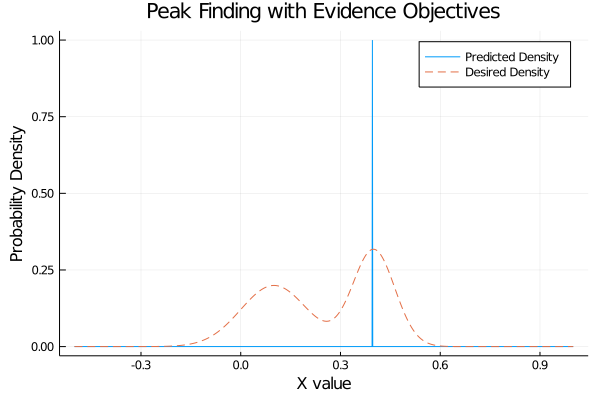
\includegraphics[width=.9\linewidth]{chapter_5_figures/evidence.png}
  \caption{Optimizing with an Evidence Objective}
\end{subfigure}%
\begin{subfigure}{.5\textwidth}
  \centering
  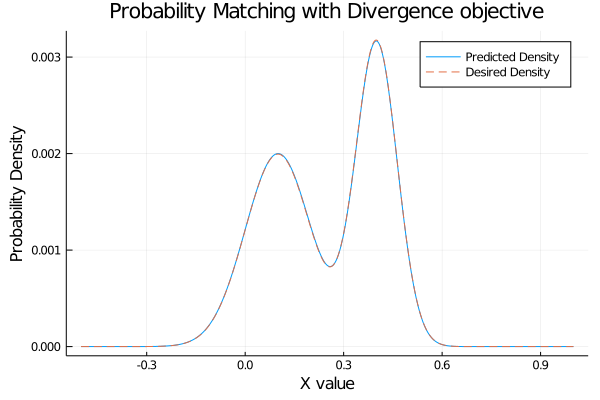
\includegraphics[width=.9\linewidth]{chapter_5_figures/divergence.png}
  \caption{Optimizing with a Divergence Objective}
\end{subfigure}
\caption{Numerical illustration of optimizing a multimodal desired distribution with an Evidence objective (Panel A) vs a Divergence Objective (panel B). The desire distribution consisted of the sum of two univariate Gaussian distributions, with means of $1$ and $4$ and variances of $1$ and $0.4$ respectively. We then optimized an expected future distribution, which also consisted of two Gaussians with free means and variances using both an Evidence and a Divergence objective. As can be seen, optimizing the Evidence Objective results in the agent fitting the predicted future density entirely to an extremely sharp peak around the mode of the desired distribution. Conversely, optimizing a divergence objective leads to a precise match of the predicted and desired distributions (panel B shows the two distributions almost precisely on top of one another). As a technical note, to be able to see both the evidence and deisre distributions on the same scale, for the evidence objective the predicted distribution is normalized but the desired distribution is not. Code for these simulations can be found at: https://github.com/BerenMillidge/origins\_information\_seeking\_exploration.}
\end{figure}
Another way we can interpret the difference between the objectives is in terms of the effect of the objective upon the predicted distribution $p(o_{1:T} | a_{1:T})$. Specifically, we can think of the divergence objective as a balance between trying to maximize the likelihood of the desired distribution under the predicted distribution, and trying to \emph{maximize} the entropy of the predicted distribution. We can think of this as the divergence objective as effectively saying `try to maximize your desires or utility while also keeping the future as broad as possible' -- i.e. keeping your options open. This can be demonstrated mathematically through the simple definition of the KL divergence,
\begin{align*}
\mathcal{L}_{divergence} &= \underset{a_{1:T}}{argmin} \, \KL[p(o_{1:T}) | a_{1:T}) || \tilde{p}(o_{1:T})] \\
&= \underset{a_{1:T}}{argmin} \, \underbrace{-\mathbb{H}[p(o_{1:T} | a_{1:T})]}_{\text{Predicted Entropy}} - \underbrace{\mathbb{E}_{p(o_{1:T} | a_{1:T})}[\ln \tilde{p}(o_{1:T})]}_{\text{Evidence Objective}}
\end{align*}

Here we see that we can express the divergence objective simply as the evidence objective plus the maximization of the entropy of the predicted distribution. In effect, the divergence objective simply includes an entropy regulariser to the standard evidence objective. Conversely, we can also express the relationship between the objectives in the other way. We can think of the evidence objective as simply trying to match the predicted and desire distribution while simultaneously \emph{minimizing} the entropy of the predicted distribution. This is straightforward to show mathematically,
\begin{align*}
\mathcal{L}_{Evidence} &= \underset{a_{1:T}}{argmax} \, \mathbb{E}_{p(o_{1:T} | a_{1:T})}[\ln \tilde{p}(o_{1:T})] \\
    &= \underset{a_{1:T}}{argmax} \, \mathbb{E}_{p(o_{1:T} | a_{1:T})}[\ln \tilde{p}(o_{1:T})\frac{p(o_{1:T} | a_{1:T})}{p(o_{1:T} | a_{1:T})}] \\
    &= \underset{a_{1:T}}{argmax} \, -\underbrace{\KL[p(o_{1:T} | a_{1:T}) || \tilde{p(o_{1:T})}]}_{\text{Divergence}} - \underbrace{\mathbb{H}[p(o_{1:T} | a_{1:T})]}_{\text{Expected Future Entropy}} \numberthis
\end{align*}

This formulation gives a straightforward intuition for the `mode-seeking' behaviour of the evidence objective. The evidence objective seeks to match the predicted and desire distribution, while also being penalized for the breadth of the predicted distribution. The best way to resolve this tension is by forming a highly peaked predicted distribution around the mode of the desire distribution so that it can cover as much probability mass as possible. 

Interestingly, differences between the two formulations generally only emerge when the desire distribution is broad and complex. Here, the divergence objective will tend to force the predicted distribution and desire distribution to match in their complexity, while the evidence distribution will seek out and focus around its mode. Another intuitive way of thinking about the distinction is that the divergence objective implicitly maximizes some sort of future empowerment, by implicitly trying to keep all future options open, by seeking to make future observations as entropic as possible. Evidence objectives, by contrast, seek the opposite. They aim for `precise futures' where the amount of future variability is as low as possible. It is straightforward to show that, unlike evidence objectives, divergence objectives can be immediately decomposed into an `extrinsic' value divergence term, and an information-seeking exploratory term,

\begin{align*}
    \KL[p(o_{1:T} | a_{1:T}) || \tilde{p}(o_{1:T})] &= \mathbb{E}_{p(o_{1:T} | a_{1:T})}[\ln \frac{p(o_{1:T} | a_{1:T})}{\tilde{p}(o_{1:T})}] \\
 &= \mathbb{E}_{p(o_{1:T} | a_{1:T})}[\ln \frac{p(o_{1:T} | a_{1:T})}{\tilde{p}(o_{1:T})}] \\
 &= \mathbb{E}_{p(o_{1:T} | a_{1:T})}[\ln \frac{p(o_{1:T},x_{1:T} | a_{1:T})}{\tilde{p}(o_{1:T})p(x_{1:T} | o_{1:T})}] \\
 &= \underbrace{\mathbb{E}_{p(x_{1:T})}\KL[p(o_{1:T} | x_{1:T})||\tilde{p}(o_{1:T})]}_{\text{Desire Divergence}} \\ &- \underbrace{\mathbb{E}_{p(o_{1:T} | a_{1:T})}\KL[p(x_{1:T} | o_{1:T})||p(x_{1:T})]}_{\text{Information Gain}} \numberthis
\end{align*}

Importantly, the property that divergence objectives give rise to directed information-seeking exploratory terms, arises directly from the previously discussed intuition that they attempt to maximize the entropy of future observations. Such information gain terms arise whenever the predicted distribution is extended to model additional latent variables or parameters. The proof of this is straightforward,
\begin{align*}
    \mathbb{H}[p(o_{1:T} | a_{1:T})] &= \mathbb{E}_{p(o_{1:T},x_{1:T} | a_{1:T})}[\ln p(o_{1:T} | a_{1:T})] \\
    &= \mathbb{E}_{p(o_{1:T},x_{1:T} | a_{1:T})}[\ln \frac{p(o_{1:T},x_{1:T} | a_{1:T})}{p(x_{1:T} | o_{1:T})}] \\ 
    &=- \underbrace{E_{p(x_{1:T})}\mathbb{H}[p(o_{1:T} | x_{1:T})]}_{\text{Likelihood Entropy}} - \underbrace{\mathbb{E}_{p(o_{1:T} | a_{1:T})}\KL[p(x_{1:T} | o_{1:T}) || p(x_{1:T})]}_{\text{Expected Information Gain}} \numberthis
\end{align*}

Put verbally, this relationship shows that to maximize the entropy of a distribution, if the distribution can be understood in terms of a latent set of variables, requires both maximizing the conditional entropy of the variable given the latent variables, while simultaneously maximizing the mutual information of the latent variables between the observed and latent variables. Intuitively, within our context, this means that to maximize the entropy of future observations, it is necessary to successfully model the relationship between these future observations and their latent states, which entails maximizing the mutual information between the latents and the observations. It is the maximization of this mutual information which undergirds the exploratory information-seeking behaviour which is manifested by divergence objectives. Conversely, the fact that evidence objectives seek to \emph{minimize} the entropy of the predicted distribution means that they implicitly seek to minimize the amount of mutual information between observation and latent variables. We can think of this as divergence objectives aim to reach a given set of goals while also learning as much as possible about the environment, in order to precisely match the two distributions. Evidence objectives, on the other hand, seek to reach their goals while learning as little as possible about the environment, and keeping the environment as regular and predictable as possible. 

Now that we have proposed and given considerable intuition for our dichotomy between evidence and divergence objectives, we look to see where these objectives appear in the literature, and how they can explain differences in exploratory behaviour between differing paradigms.

\subsection{Control as Inference}

It is straightforward to show that the control as inference, and variational inference objectives are bounds upon the evidence objective. Put simply, we have that control as inference aims to solve the inference problem of inferring an action distribution given a desired set of observations. Specifically, we seek to obtain the distribution $p(a_{1:T} | \tilde{o}_{1:T})$ where we use $\tilde{o}$ to denote a set of hypothetical `optimal' actions which have been conditioned upon. To find this posterior, we use a variational approximation by defining the variational density $q(a_{1:T})$ and optimizing the following variational lower bound,
\begin{align*}
    \KL[q(a_{1:T} || p(a_{1:T} | \tilde{o}_{1:T})] &= \KL[q(a_{1:T} || \tilde{p}(o_{1:T}, a_{1:T})] - \ln p(o_{1:T}) \\
    &\geq \underbrace{\KL[q(a_{1:T} || \tilde{p}(o_{1:T}, a_{1:T})]}_{\text{CAI Objective}}
\end{align*}
Which serves as the control as inference objective. It is then straightforward to show that this objective serves as a bound on an evidence objective,
\begin{align*}
    \underset{a_{1:T}}{argmax} \, \ln \tilde{p}(o_{1:T}) &= \underset{a_{1:T}}{argmax} \, \ln \int dx \, \tilde{p}(o_{1:T} x_{1:T}) \\
    &= \underset{a_{1:T}}{argmax} \, \ln \int dx \,  \frac{\tilde{p}(o_{1:T} x_{1:T})q(a_{1:T})}{q(a_{1:T})} \\
    &\geq \underset{a_{1:T}}{argmax} \, \mathbb{E}_{q(a_{1:T})}[\ln \frac{\tilde{p}(o_{1:T},a_{1:T})}{q(a_{1:T})}] \\
    &\geq \underset{a_{1:T})}{argmin} \, - \KL[q(a_{1:T}) || \tilde{p}(o_{1:T}, a_{1:T})] \\
    &= \geq \mathcal{L}_{CAI} \numberthis
\end{align*}

And thus we can see that the control as inference framework optimizes a variational bound on the evidence objective. This straightforwardly explains why control as inference approaches do not give rise to directed, information-seeking exploration, but rather instead only induce \emph{random} action entropy maximizing exploration terms. This \emph{random} exploration, while highly efficient in many contemporary dense-reward reinforcement learning benchmark tasks, where a random policy often suffices to cover enough of the state space, it is increasingly ineffective in extremely high dimensional, and sparse reward environments.

\subsection{KL Control}

Another control method in the literature that has been applied, and studied fairly extensively is KL control. Although not as widely used in reinforcement learning, it is often implicit optimized in control tasks, and has deep relationships with the beginning of the control as inference approach, as well as more esoteric path integral methods. Moreover, it has recently seen renewed application in deep reinforcement learning approaches such as state-marginal matching of \citep{lee2019efficient}. KL control, as the name implies, chooses control to minimize the KL divergence between the current state and a set of desired states, leading to the following objective function,
\begin{align*}
    \mathcal{L}_{KL} = \underset{a_{1:T}}{argmin} \, \, \KL[p(x_{1:T}) || \tilde{p}(x_{1:T})] \numberthis
\end{align*}
Here we have used $x$ instead of $o$ to denote that KL control has typically only been applied to fully-observed Markovian MDP environments as opposed to full POMDP dynamics. As such, while the KL control objective is clearly just the divergence objective,  its superior exploratory capabilities have not been significantly explored in the literature due to the only applications currently being in fully observable environments while the information-seeking exploratory terms require the extension to hidden variable models. Another interesting point is that the objective in continuous time active inference in predictive coding models can also be as a KL divergence between a desired `set-point' and a currently observed point, and is thus an instance of KL control. However, these models also do not handle latent variable models, and thus also do not manifest the full exploratory capabilities of divergence objectives.

\subsection{Active Inference}

Given that we know from previously, that the expected free energy contains an information gain term, which gives rise to the information-seeking exploratory behaviour of active inference agents, it is worth investigating the relationship of the EFE to evidence and divergence functionals. Recall, from the previous section that the EFE formed neither an upper nor a lower bound upon the log model evidence, but instead formed an upper bound when the posterior divergence was greater than the information gain term, and a lower bound otherwise, with the goal of eventually converging directly to the log model evidence in the case that both of these terms become zero. Noting that the log model evidence simply, as the name suggests, is the evidence, objective, we can rewrite this in terms of our new understanding as,

\begin{align*}
    \underbrace{\mathbb{E}_{q(o,x)}[\ln \tilde{p}(o)]}_{\text{Evidence Objective}} &= \underbrace{\mathbb{E}_{q(o,x)}[\ln q(x) - \ln \tilde{p}(o,x)]}_{\text{EFE}} +  \underbrace{\mathbb{E}_{q(o)}\KL[q(x | o) || q(x)]}_{\text{Information Gain}} - \underbrace{\mathbb{E}_{q(o)}\KL[q(x | o) || p(x | o)]}_{\text{Posterior Divergence}} \\
    &\implies \underbrace{\mathbb{E}_{q(o,x)}[\ln \tilde{p}(o)]}_{\text{Evidence Objective}} \geq \underbrace{\mathbb{E}_{q(o,x)}[\ln q(x) - \ln \tilde{p}(o,x)]}_{\text{EFE}} \\
    &\text{If} \, \,  \underbrace{\mathbb{E}_{q(o)}\KL[q(x | o) || q(x)]}_{\text{Information Gain}} \geq \underbrace{\mathbb{E}_{q(o)}\KL[q(x | o) || p(x | o)]}_{\text{Posterior Divergence}} \numberthis
\end{align*}
so that the EFE does not stand in a straightforward relationship as bound in any specific direction on the evidence objective. Nevertheless, since the EFE contains an information gain term to be maximized, as do divergence objectives, we might expect to obtain a straightforward relationship between the EFE and the divergence objective. We can write out the relationship between the divergence objective and the EFE as follows,

\begin{align*}
    \underbrace{\KL[p(o) || \tilde{p}(o)]}_{\text{Divergence Objective}} &= \mathbb{E}_{p(o)}[\ln \frac{ \int dx p(o,x)}{\tilde{p}(o)}] \\
    &= \mathbb{E}_{p(o)}[\ln \frac{ \int dx p(o,x)q(x | o)q(o,x)}{\tilde{p}(o)q(x | o)q(o,x)}] \\
    &\leq \mathbb{E}_{p(o)}[\ln \frac{ \int dx p(o,x)q(o,x)}{\tilde{p}(o)q(x | o)q(o,x)}] \\
    &\leq \mathbb{E}_{p(o)}[\ln \frac{ \int dx p(o,x)q(o | x)q(x)}{\tilde{p}(o)q(x | o)q(x | o)q(o)}] \\
    &\leq \underbrace{\mathbb{E}_{p(o)q(x | o)}[\ln q(x) - \ln q(x | o)- \ln \tilde{p}(o)]}_{\text{EFE}}- \underbrace{\mathbb{E}_{p(o)}\KL[q(x | o)||p(o,x)]}_{\text{VFE}} \\ &+\underbrace{\mathbb{E}_{q(x | o)p(o)}\KL[q(x | o) || q(x)]}_{\text{Information Gain}} \numberthis
\end{align*}

Here we see that the EFE can be expressed in terms of the divergence objective, an information gain term, and, interestingly, the variational free energy.  In effect, the divergence objective consists of the EFE, the VFE, and an information gain term. Specifically, the EFE becomes an upper bound on the divergence objective when the information gain term is greater than the variational free energy. This is similar to previously where we saw that the EFE became a bound on the evidence when the information gain is less than the posterior divergence. It is thus clear that the EFE objective does not serve as a valid and consistent bound on either of the divergence or the evidence objectives. Similarly, we can express the EFE directly in terms of the divergence objective as follows,

\begin{align*}
    \underbrace{\KL[p(o) || \tilde{p}(o)]}_{\text{Divergence Objective}} &= \mathbb{E}_{q(x | o)p(o)}\KL[p(o)q(o,x) || \tilde{p}(o)q(o,x)] \\
    &= \mathbb{E}_{q(x | o)p(o)}\KL[p(o)q(o|x)q(x) || \tilde{p}(o)q(x | o)q(o)] \\
    &= \underbrace{\mathbb{E}_{q(x | o)p(o)}[\ln q(x) - \ln \tilde{p}(o) - \ln q(x | o)]}_{\text{EFE}} + \underbrace{\mathbb{E}_{p(o)}\KL[q(x | o) || q(x)]}_{\text{Information Gain}} - \underbrace{\mathbb{H}[p(o)]}_{\text{Marginal Entropy}} \numberthis
\end{align*}
Where we see that the divergence objectives simply is the EFE plus an information gain term, minus the marginal or predicted entropy term. As such, even within this framework, the mathematical origin and the behaviour of the EFE remains unclear since the EFE does not form consistent bounds on either objective, but instead oscillates above and below both.

\subsection{Action and Perception as Divergence Minimization}
A recent framework, inspired by active inference and advances in deep reinforcement learning, which aims to unify perception and action under a single framework is Action and Perception as Divergence Minimization \citep{hafner2020action} (APDM). This framework proposes that both action and perception can be modelled as an agent trying to mininimize a divergence functional between two distributions an `actual' distribution $A(x,o)$, and a target distribution $T(x,o)$. 

\begin{align*}
    \mathcal{L}_{APDM} &= \KL[A(x,o) || T(x,o)] \\
    &= \underbrace{\mathbb{E}_{A(x)}\KL[A(o | x) || T(o)]}_{\text{Realizing Latent Preferences}} - \underbrace{\mathbb{E}_{A(x,o)}[\ln T(x | o) - \ln A(x)]}_{\text{Information Bound}} \numberthis
\end{align*}

\begin{align*}
    -\underbrace{\mathbb{E}_{A(x,o)}[\ln T(x | o) - \ln A(x)]}_{\text{Information Bound}} &= -\mathbb{E}_{A(x,o)}[\ln T(x | o) - \ln A(x) + \ln A(x | o) - \ln A(x | o)] \\
    &= - \underbrace{\mathbb{E}_{A(o)}\KL[A(x | o) || A(x)]}_{\text{Information Gain}} + \underbrace{\mathbb{E}_{A(o)}\KL[A(x |o) || T(x | o)]}_{\text{Posterior Divergence}} \numberthis
\end{align*}
By expressing this bound explicitly, we can see how it is an upper bound on the information gain, since the posterior divergence is always positive. The tightness of the bound then depends on how closely the actual and target distributions match. In general, we can use this approach to write out a full expression for the divergence objective between two joint distributions over both observations and latent variables.
\begin{align*}
    \mathcal{L}_{joint} &= \underset{a}{argmin} \, \KL[p(o,x) || \tilde{p}(o,x)] \\
    &= \underbrace{\mathcal{E}_{p(x)}\KL[p(o| x) || \tilde{p}(o)]}_{\text{Likelihod Divergence}} - \underbrace{\mathbb{E}_{p(o,x)}[\ln \tilde{p}(x | o) - \ln p(x)]}_{\text{Information Bound}} \\
    &= \underbrace{\mathbb{E}_{p(x)}\KL[p(o| x) || \tilde{p}(o)]}_{\text{Likelihod Divergence}} -  \underbrace{\mathbb{E}_{p(o)}\KL[p(x | o) || p(x)]}_{\text{Information Gain}} + \underbrace{\mathbb{E}_{p(o)}\KL[p(x |o) || \tilde{p}(x | o)]}_{\text{Posterior Divergence}} \numberthis
\end{align*}
 
In effect, we see that minimizing the divergence between two joint distributions requires the minimizations of both the likelihood divergence \emph{and} the posterior divergence, while also requiring the maximization of the information between posterior and prior of the first term in the joint KL.

It is also straightforward to relate this joint divergence to the divergence objective, which is the divergence between marginals instead of joints. 
\begin{align*}
    \underbrace{\KL[p(o,x) || \tilde{p}(o,x)]}_{\text{Joint Divergence}} &= \KL[p(o)p(x|o)||\tilde{p}(x |o)\tilde{p}(x|o)] \\
    &= \underbrace{\KL[p(o) || \tilde{p}(o)]}_{\text{Divergence Objective}} + \underbrace{\mathbb{E}_{p(o)}\KL[p(x | o)||\tilde{p}(x|o)]}_{\text{Posterior Divergence}} \\
    &\geq \underbrace{\KL[p(o) || \tilde{p}(o)]}_{\text{Divergence Objective}} \numberthis
\end{align*}
Since the posterior divergence is always positive (as a KL divergence), we observe that the joint divergence is simply an upper bound on the divergence objective. Since the divergence is minimized, this bound is in the correct direction, and thus minimizing the joint divergence is a reasonable proxy for minimizing the marginal divergence objective. By minimizing the joint, it implicitly encourages agents to minimize both the marginal divergence as well as the divergence between the predicted and desired posterior distributions.

While the generic APDM divergence, as just a divergence of joints, is straightforwardly an upper bound on the divergence objective, we show that under the common definitions of the actual and target distributions, the APDM divergence can also be understood as a lower bound on the evidence objective, thus providing a bridge between the two objectives. Although the actual and target distributions can be defined differently depending on the objective you desire to reproduce, one canonical form of the actual and target distributions, which can reproduce control as inference as well as variational perceptual inference is as follows. We define the actual distribution to be the combination of the `real' data distribution $p(o)$ and also a variational belief distribution $q(x | o)$ such that $A(o,x) = q(x | o)p(o)$. Similarly, we define the target distribution to be the product of the agent's veridical generative model $p(o,x)$ and the exogenous desire distribution $\tilde{p}(o)$ such that $T(o,x) = p(o,x)\tilde{p}(o)$. This target distribution is valid as long as the ultimate objective is optimized via gradients of the divergence, which does not require that the target distribution be normalized. Under this definition of the actual and target distributions, the APDM objective becomes,

\begin{align*}
    \mathcal{L}_{APDM} = \KL[q(x | o)p(o) || p(o,x)\tilde{p}(o)] \numberthis
\end{align*}
In the case of known observations in the past, we assume that the data distribution becomes points around the actually observed observations $p(o) = \delta(o = \hat{o})$ while the desire distribution becomes uniform -- as there is little use for control in having desires about the unalterable past. Under these assumptions, the APDM objective simply becomes the ELBO or the negative free energy, thus replicating perceptual inference. However, on inputs in the future, the data distribution becomes a function of action (since actions can change future observations) and the desire distribution becomes relevant, thus allowing the minimization of the APDM functional to underwrite control. To gain a better intuition for the interplay of perception and control in the APDM functional, we showcase the following decomposition,
\begin{align*}
    \mathcal{L}_{APDM} &= \KL[q(x | o)p(o) || p(o,x)\tilde{p}(o)] \\
    &= \underbrace{\mathbb{E}_{p(o)}\KL[q(x | o) || p(o,x)]}_{\text{ELBO}} + \underbrace{\KL[p(o)||\tilde{p}(o)]}_{\text{Divergence Objective}} \numberthis
\end{align*}

which demonstrates that the APDM objective effectively unifies action and perception by summing together a perceptual objective (VFE) with the divergence objective for control. This confirms the previous finding that the APDM objective forms an upper bound on the divergence objective since the ELBO, as a KL divergence, is bounded below by 0. We also observe that this form of the APMD objective is also approximately a lower bound on the expected evidence objective, thus providing a link between the two objectives.
\begin{align*}
    \mathbb{E}_{p(o | a)}[\ln \tilde{p}(o)] &= \mathbb{E}_{p(o | a)}[\ln \int dx \, \tilde{p}(o,x)] \\
    &= \mathbb{E}_{p(o | a)}[\ln \int dx \, \frac{\tilde{p}(o,x)q(x|o)p(o,x)}{q(x | o)p(o,x)}] \\
    &\geq \mathbb{E}_{p(o)q(x | o)}[\ln \frac{\tilde{p}(o,x)p(o,x)}{q(x|o)p(o,x)}] \\
    &\geq \mathbb{E}_{p(o)q(x | o)}[\ln \frac{\tilde{p}(o)\tilde{p}(x|o)p(o,x)}{q(x|o)p(o)p(x|o)}] \\
    &\geq -\underbrace{\mathbb{E}_{p(o)q(x | o)}[\KL[q(x|o)p(o)||p(o,x)\tilde{p}(o)]}_{\text{APDM Objective}} +\underbrace{\mathbb{E}_{p(o)q(x|o)}[\ln \tilde{p}(x|o) - \ln p(x|o)]}_{\text{Posterior Divergence Bound}}\\
    &\approx \geq \underbrace{\mathbb{E}_{p(o)q(x | o)}[\KL[q(x|o)p(o)||p(o,x)\tilde{p}(o)]}_{\text{APDM Objective}} \numberthis
\end{align*}

Which is approximately equal to the APDM objective under the condition that the posterior divergence bound between desire posterior $\tilde{p}(x | o)$ and true posterior $p(x | o)$ is small.

\section{Towards a General Theory of Mean-Field Variational Objectives for Control}

Now that we understand the division of objectives for control into two classes of evidence and divergence functionals, we can start to try to understand the full possibilities of the space of potential objectives. Here, in this final section of Chapter 5, we try to present precisely such a taxonomy. We focus specifically on `mean-field' variational objective functionals, meaning that we can split the objective into a number of independent objectives for each time-step of a trajectory which can be minimized independently. Crucially, such a mean-field assumption is also made in the traditional reinforcement learning paradigm, where it is a necessary precondition for the Bellman equation, and also is standard in the control as inference framework as well.

While the division into divergence and evidence objectives is clearly important, it cannot be the full story. Recall that one of the key differences between control as inference and active inference discussed earlier, was not just the objective of the EFE vs the FEF, but also the way value was encoded into the inference procedure. Control as inference encoded value via an additional set of `optimality variables' which were augmentations to the graphical model, and did not interact with any previously existing variables. Active inference, by contrast, encoded value directly through a biased generative model of the observations \footnote{Active inference can also be formulated with biased states, see  \citep{da2020active}}. We call the method used by control as inference, which does not affect any currently existing variable an \emph{exogenous} encoding of value, while the method used by active inference, since it encodes value directly into the model itself, we call an \emph{endogenous} encoding. Exogenous and Endogenous encodings of value provide an orthogonal dimension of objective variablility on top of the evidence-divergence dichotomy, since clearly one can have an evidence, or a divergence objective with both an endogenous or an exogenous value encoding. Finally, the actual specifics of the generative model used clearly affects the variational objective irrespective of whether it is an evidence or divergence objective, or uses an endogenous or exogenous value encoding. For instance, whether we consider latent states, or various different types of model parameters in the generative model leads to a different objective functional. 

We thus see that we can break down the landscape of potential mean field objective functionals for control into three orthogonal dimensions. 
\begin{itemize}
    \item Whether an evidence or divergence functional is used.
    \item Whether value is encoded exogenously, or endogenously.
    \item The generative model underlying the objective functional.
\end{itemize}

Under different values for each of these dimensions, the objective functional that is specified changes in a straightforward and principled manner. Thus, our scheme allows the direct derivation of any given functional, and an understanding of its decompositions, and hence the behaviour it induces, for any choice of these variables. While we have covered the effect of choosing an evidence or a divergence functional previously, we have not yet been explicit about the effect of the other two dimensions. In this section, we explore the effects of these additional dimensions of design choice in more detail.


\subsection{Encoding Value}

However, the need to encode goals or desires into the inference procedure immediately introduces design choices of how exactly this is to be done. We argue that these design choices can first be split along two orthogonal axes -- firstly, whether goals are encoded exogenously as an additional input to the inference process, or endogenously through fundamentally biasing one or more aspects of the inference model. The second axis of variation is whether goals and desires enter the inference procedure through the generative model or the variational distribution. Making different design choices here produces a variety of different variational algorithms for control.

If goals are encoded through the generative model, then whether the goals are encoded exogenously or endogenously is the primary distinction between the formalisms of control-as-inference and active inference. On the other hand, encodings goals through the variational model instead leads to novel algorithms which generally have not been much explored in the literature. Encoding goals exogenously through the variational distribution leads to a variational bound similar to control-as-inference but with an extrinsic value term with a reversed-KL-divergence which thus exhibits mode-seeking rather than mean-seeking behaviour, which is related to pseudolikelihood methods \citep{peters2007reinforcement} in variational reinforcement learning. Encoding endogenous goals through the variational distribution leads to a novel class of reverse-active-inference algorithms which minimize a variational divergence between a biased approximate posterior and a veridical generative model. 

\subsubsection{Exogenous Value: Maximum-Entropy RL}

To encode goals exogenously into the generative model, we must augment the POMDP graphical model with additional optimality variables $\Omega_{t:T}$. The idea here is that the optimality variables are binary bernoulli variables which mark whether a trajectory is optimal from the current state where the probability of optimality is often set to the exponentiated reward $p(\Omega_t=1) \propto exp(r_t)$ so that $\ln p(\Omega_t = 1) = r_t$. Adaptive actions are then inferred by first assuming that the agent has acted optimally into the future, and then inferring the actions that would be consistent with that belief -- i.e. we wish to infer the posterior $p(a_{t:T} | x_{t:T}, \Omega_{t:T}=1)$. This posterior can then be approximated by minimizing the augmented variational bound:
\begin{align*}
    \mathcal{F}_\Omega &= \KL \Big( q(x_t, a_t | o_t) \Vert p(o_t, x_t, a_t, \Omega_t) \Big) \geq \KL \Big(q(x_t, a_t | o_t) \Vert p(o_t, x_t, a_t | \Omega_{t:T}) \Big) \numberthis
\end{align*}

By splitting apart this bound into its constituent parts, we can investigate the expected behaviour of agents which act so as to minimize the bound.
\begin{align*}
    \mathcal{F}_\Omega &= \KL \Big(q(x_t, a_t | o_t) \Vert p(o_t, x_t, a_t, \Omega_t) \Big) \\
    &= \KL \Big( q(a_t | x_t)q(x_t | o_t) \Vert p(\Omega_t | x_t, a_t)p(o_t | x_t)p(a_t | x_t)p(x_t | x_{t-1}, a_{t-1}) \Big) \\ 
    &= \underbrace{- \mathbb{E}_{q(x_t,a_t | o_t)}\big[\ln p(\Omega_t | x_t, a_t) \big]}_{\text{Extrinsic Value}} - \underbrace{\mathbb{E}_{q(x_t,a_t | o_t)}\big[\ln p(o_t | x_t) \big]}_{\text{Observation Ambiguity}} + \underbrace{\mathbb{E}_{q(x_t | o_t)}\big[ \KL \Big(q(a_t | x_t) \Vert p(a_t | x_t) \Big) \big]}_{\text{Action Divergence}} \\ &+ \underbrace{\KL \Big(q(x_t | o_t) \Vert p(x_t | x_{t-1}, a_{t-1}) \Big)}_{\text{State Divergence}} \numberthis
\end{align*}

The bound thus splits into four separate and identifiable terms -- extrinsic value, observation ambiguity, action divergence, and state divergence. The first extrinsic value term corresponds to the expected external rewards given by the environment. This is due to the definition of optimality that $\ln p(\Omega_t | x_t, a_t) \triangleq r(x_t, a_t)$ so that the extrinsic value is simply the expected reward of a given state-action pair. By minimizing the negative expected reward, we wish to maximize the expected reward on a given time-step. This is identical to the standard reinforcement learning objective of reward maximization so that if $\mathcal{F}_\Omega$ only contained the extrinsic value term, it would be exactly equivalent to reinforcement learning except that the expectation is taken with respect to the agent's beliefs over states and actions rather than the true environmental transition dynamics.

The observation ambiguity term $\mathbb{E}_{q(x_t,a_t | o_t)}\big[\ln p(o_t | x_t) \big]$ grants a bonus to agents for reaching areas of state-space with a high expected likelihood, that is areas where the state-observation mapping is highly precise. In effect, if the agent must learn a likelihood mapping,  this discourages exploration by granting bonuses for staying in regions already well characterised. This term only arises in the POMDP setting due to the addition of a likelihood term in the generative model. The third term is the action divergence which is to be minimized, and penalizes the agent for the divergence between its variational policy $q(a_t | x_t)$ and its prior policy $p(a_t | x_t)$. If the prior policy is assumed to be uniform such that $p(a_t | x_t) \triangleq \frac{1}{|\mathcal{A}|}$ where $|\mathcal{A}|$ is the cardinality of the action space in discrete action-spaces, and $p(a_t | x_t) \triangleq \textit{Unif}(a_{min},a_{max})$ in continuous action spaces with a minimum and maximum action value, then this action divergence term reduces to the negative expected action entropy $-\mathbb{E}_{q(x_t | o_t)}\big[\mathcal{H}[q(a_t | x_t)]\big]$. The final term is the state divergence, so that the agent tries to minimize the divergence between its variational posterior over the state and the prior state expected under the generative model. If the transition model is learnt, this leads it to prioritising transitions with known dynamics, again causing the agent to primarily confine itself to regions of the state-space it has already modelled well. In the MDP setting, without observations, this term vanishes since the variational posterior $q(x_t | o_t)$ becomes the variational prior $q(x_t)$ which is often assumed equal to the generative prior $p(x_t | x_{t-1},a_{t-1})$. Thus in the case of an MDP with a uniform action prior we obtain the maximum-entropy RL objective:
\begin{align*}
    \mathcal{F}_{maxent} = - \mathbb{E}_{q(x_t,a_t)}\big[\ln p(\Omega_t | x_t, a_t) \big] - \mathbb{E}_{q(x_t)}\big[\mathcal{H}[q(a_t | x_t)]\big] \numberthis
\end{align*}

Which induces agents both to maximize expected rewards while also maximizing the policy entropy. Intuitively this means that the agent should try to maximize rewards while acting as randomly as possible (maximizing entropy). This policy entropy term thus provides a crude bonus for random exploration and often helps prevents the commonly-observed phenomenon of `policy collapse' \citep{fujimoto2018addressing} whereby reinforcement learning agents will often rapidly learn to put all probability mass onto a single action, thus preventing other actions from being taken, hindering exploration and long-term performance. Interestingly, when extended to the POMDP case with learnt transition and likelihood models, this formalism gives rise to additional observation-ambiguity and state-divergence terms which serve to further disincentivise exploration by penalising moving too far from the prior predicted state and giving bonuses for highly predictable likelihoods. Intuitively we can think of these extra terms as trying to do away with the additional uncertainty induced by the POMDP setting, so the agent confines itself to the region which is as close to an MDP as possible.

\subsubsection{Endogenous Value: Active Inference}

While maximum entropy reinforcement methods can be derived by encoding goals exogenously to the generative model through the use of additional `optimality variables', it is also possible to encode goals \textit{endogenously} by directly biasing some aspect of the generative model towards preferred outcomes. Intuitively, we can think of the difference as follows. With exogenous optimality variables, we possess a veridical generative model outputting the likely and unbiased trajectories for a given series of actions. We then `shift' these trajectories to converge on the goal by conditioning on the optimality variables, and then infer the actions consistent with the shifted trajectories. By contrast, active inference endogenously encodes goals by biasing the model so that instead of a veridical generative model which generates trajectories that are then shifted, instead we have a \emph{biased} generative model which directly outputs a biased trajectory of observations $\Tilde{o}_{t:T}$ converging on the goal, which can then be used to infer the actions consistent with this biased trajectory. In this manner, instead of proposing additional optimality variables, we directly posit a biased generative model $\tilde{p}(o_t, x_t, a_t)$ and optimise the biased variational bound:
\begin{align*}
    \mathcal{F}_{likelihood-AIF} &= \KL \Big( q(x_t, a_t | o_t) \Vert \tilde{p}(o_t, x_t, a_t) \Big) \\
    &= \KL \Big( q(a_t | x_t)q(x_t | o_t) \Vert \tilde{p}(o_t | x_t) p(x_t | x_{t-1},a_{t-1})p(a_t | x_t)  \Big) \\
    &= - \underbrace{\mathbb{E}_{q(x_t | o_t)} \big[\ln \tilde{p}(o_t | x_t) \big]}_{\text{Extrinsic Value}} + \underbrace{\mathbb{E}_{q(x_t | o_t)}\big[ \KL \Big(q(a_t | x_t) \Vert p(a_t | x_t) \Big) \big]}_{\text{Action Divergence}} \\ &+ \underbrace{\KL \Big(q(x_t | o_t) \Vert p(x_t | x_{t-1}, a_{t-1}) \Big)}_{\text{State Divergence}} \numberthis
\end{align*}

This variational bound decomposes into three terms as can be seen above. The first, extrinsic value, is such because it is the biased probability of observations expected under the variational distribution. If we assume that the biased generative model is influenced by the external rewards in the environment, to allow for consistency with reinforcement learning and the maximum-entropy RL framework such that $\ln \tilde{p}(o_t | x_t) \propto exp(r(x_t)$ then this first term reduces to minimizing the expected sum of negative rewards, or maximising expected rewards. The other two action-divergence and state-divergence terms are equivalent to the terms in the maximum entropy bound above, except that the active inference bound is lacking the `observation ambiguity' term. This is because exogenously encoding goals adds an additional set of optimality variables to the variational bound, thus maintaining a distinction between veridical observations and biased optimality variables, while endogenously encoding goals needs to `hijack' at least one degree of freedom in the bound in order to encode the goals directly. Here the observation ambiguity term has effectively been hijacked by being biased with reward to instead encode the extrinsic value.

Interestingly, the choice of encoding goals endogenously also gives an additional set of choices of how to bias the generative model. The key choice is between having a biased likelihood, as done above, or a biased marginal and posterior. This decomposition is shown below:
\begin{align*}
     \mathcal{F}_{marginal-AIF} &= \KL \Big( q(x_t, a_t | o_t) \Vert \tilde{p}(o_t, x_t, a_t) \Big) \\
    &= \KL \Big( q(a_t | x_t)q(x_t | o_t) \Vert \tilde{p}(o_t)\tilde{p}(x_t | o_t) p(a_t | x_t)  \Big) \\
    &= - \underbrace{\mathbb{E}_{q(x_t | o_t)} \big[\ln \tilde{p}(o_t) \big]}_{\text{Extrinsic Value}} + \underbrace{\mathbb{E}_{q(x_t | o_t)}\big[ \KL \Big(q(a_t | x_t) \Vert p(a_t | x_t) \Big) \big]}_{\text{Action Divergence}} + \underbrace{\KL \Big(q(x_t | o_t) \Vert \tilde{p}(x_t | o_t) \Big)}_{\text{Biased State Divergence}} \numberthis
\end{align*}

Here, we assume that $\ln \tilde{p}(o_t) \propto exp(r(o_t))$ such that the extrinsic value term is again directly equal to the rewards. An interesting difference is that the biased state-divergence is now between the variational posterior and the biased state posterior, which represents the posterior over states that would be observed given the biased observations. This gives this second term also the flavour of an extrinsic value as the goal is not only to maximize rewards but match the veridicial variational distribution to the biased state distribution induced by the desired observations

Alternatively, it is also possible to consider encoding the bias into the \emph{states} $\tilde{p}(x_t)$ instead of the observations. In this case, we obtain the following objective functional:
\begin{align*}
\label{state_AIF}
         \mathcal{F}_{state-AIF} &= \KL \Big( q(x_t, a_t | o_t) \Vert \tilde{p}(o_t, x_t, a_t) \Big) \\
    &= \KL \Big( q(a_t | x_t)q(x_t | o_t) \Vert p(o_t | x_t) \tilde{p}(x_t) p(a_t | x_t)  \Big) \\
    &= \underbrace{\KL \Big( q(x_t | o_t) \Vert \tilde{p}(x_t) \Big)}_{\text{Extrinsic Value}} - \underbrace{\mathbb{E}_{q(x_t,a_t | o_t)}\big[\ln p(o_t | x_t) \big]}_{\text{Observation Ambiguity}} + \underbrace{\mathbb{E}_{q(x_t | o_t)}\big[ \KL \Big(q(a_t | x_t) \Vert p(a_t | x_t) \Big) \big]}_{\text{Action Divergence}} \numberthis
\end{align*}

In this case, we have regained the observation-ambiguity term and instead the state-divergence term has been `hijacked' by the rewards to become the extrinsic value term, which has become the divergence between predicted and desired states. 

Given that there exist these two design choices of whether to encode goals exogenously or endogenously and which lead to subtly different objectives, a natural question to ask is what are the relative advantages and disadvantages of the two methods? What trade-offs exist and where might each be useful? In general, the primary practical difference between the methods is that by endogenously encoding rewards, the agent loses a degree of freedom, which manifests itself as the loss of an observation ambiguity term if the goals are encoded through biased observations, or the loss of the state-divergence term if the goals are encoded as a desired state distribution. These additional terms tend to discourage exploration by causing the agent to remain in areas with known mappings, so that by disabling them endogenous goals tend to encourage exploration. On the other hand, by keeping to well-known regions where the POMDP behaves like an MDP, the exogenous goals method enforces a greater conservative bias towards safety, which may be especially useful in settings where exploration is costly, satisficing policies are easy to find, or in policies learnt in an offline or imitation-learning setting where venturing outside of the training distribution can have deleterious effects on the policy.

There are also important philosophical and representational differences between the two. On a representational note, although in the derivations above both the optimality variable and the biased generative model have been defined in terms of exponentiated reward, this is not necessarily the case. Since in the endogenous encoding case, the goals are encoded directly as prior distributions into the generative model, it is possible to model complex and potentially nonstationary goals distributions in this manner. However, due to the optimality variables being binary, and conditioned upon, this may constrain their representational power compared to the endogenous method, although in practice this difference may be negligible as although the variables themselves are binary, the probability of optimality being one, can be defined as an arbitrary function of the states, actions or observations. Thus in practice, there may be little representational difference between the two methods, except that the endogenous case has a slightly simpler intuitive justification as directly specifying a desired distribution over states or observations.

The difference between exogenous and endogenous encodings of value also has significant philosophical import. Exogenous encodings, by adding desires on top of an unbiased generative model maintain a clean distinction between veridical perception and action selection, and goals. This maintains the core modularity thesis of much work in artificial intelligence that perception, and action selection should be kept separate such that first a veridical world-model is constructed which tries to accurately model the world, then given a set of arbitrary goals, a general-purpose planner or policy can be utilised or learnt to enable the agent to achieve these goals. This approach corresponds to the classical perceive-(value)-plan-act cycle in cognitive science and maintains separate modules for a goal-agnostic perceptual system, a goal-agnostic planner or action-selection mechanism, and then a set of goals which are not intrinsic to the agent but which are constructed or handed-down from on high. Endogenous encoding methods, by contrast, tend to blur the boundaries between these sytems, since goals are encoded and adaptive actions are selected through a process of \emph{biased} perception and inference whereby an agent does not first infer a true trajectory, compares it to its goals, and then tries to match the too, instead it simply sees a biased trajectory leading to its goals and then acts consonantly with what it sees. This view has close links to embodied and enactivist views in philosophy and cognitive science which stress that rather than distinct modular systems of perception, valuation, and action there is instead a single combined system or sensorimotor loop which directly acts on sensorimotor contingencies in an adaptive fashion \citep{baltieri2018modularity}.

\subsubsection{Encoding Value into the Variational Distribution}

Previously, we have encoded values either exogenously or endogenously into the \emph{generative model} of the agent. In the case of endogenous encodings,  this means that the agent makes biased predictions, rather than forming biased inferences. However, it is also possible to consider and investigate what happens if instead values were encoded into the variational distribution so that the agent's inference procedure rather than model is biased. We first consider the case of exogenously encoded goals. This requires that the variational distribution is augmented with binary optimality variables, just like the generative model was previously giving $q(a_t, x_t,\Omega_t | o_t)$. From this we can write the relevant free energy functional:
\begin{align*}
\label{exogenous_goals_equation}
    \mathcal{F}_{q\Omega} &= \KL \Big( q(a_t, x_t, \Omega_t | o_t) \Vert p(o_t, x_t, a_t) \Big) \\
    &= \KL \Big( q(\Omega_t | x_t, a_t)q(a_t | x_t)q(x_t | o_t) \Vert p(o_t | x_t)p(a_t | x_t)p(x_t | x_{t-1},a_{t-1}) \Big) \\
    &=  \underbrace{\mathbb{E}_{q(x_t,a_t | o_t)}\big[\ln q(\Omega_t | x_t, a_t) \big]}_{\text{Extrinsic Value}} - \underbrace{\mathbb{E}_{q(x_t,a_t | o_t)}\big[\ln p(o_t | x_t) \big]}_{\text{Observation Ambiguity}} + \underbrace{\mathbb{E}_{q(x_t | o_t)}\big[ \KL \Big(q(a_t | x_t) \Vert p(a_t | x_t) \Big) \big]}_{\text{Action Divergence}} \\ &+ \underbrace{\KL \Big(q(x_t | o_t) \Vert p(x_t | x_{t-1}, a_{t-1}) \Big)}_{\text{State Divergence}} \numberthis
\end{align*}

We see that the resulting functional, under the assumption that $\ln q(\Omega | x_t, a_t) \propto exp(r(x_t, a_t)$, is exactly equivalent to the functional obtained for the exogenously encoded generative model, up to a sign difference in the extrinsic term which can be finessed without loss of generality by inverting the sign of the reward function. We thus see that, if values are exogenously encoded, it does not matter which distribution they are primarily encoded through. Intuitively this is because since the veridical distributions are maintained through endogenous coding, they are unaffected by the encoding of value into them, thus which one to choose has no effect overall up to a trivial sign difference which can be easily finessed through negatively encoding reward.

When rewards are endogenously encoded, however, the resulting functionals are not equivalent. We first show this with a biased-state functional which should be compared to Equation \ref{exogenous_goals_equation}, where we directly bias the state-inference part of the variational functional so as to preferentially infer being in desired states from a given observation $\tilde{q}(a_t, x_t | o_t) \triangleq q(a_t | x_t) \tilde{q}(x_t | o_t)$. Through this decomposition we obtain the functional:
\begin{align*}
    \mathcal{F}_{state-q-AIF} &= \KL \Big( \tilde{q}(x_t, a_t | o_t) \Vert p(o_t, x_t, a_t) \Big) \\
    &= \KL \Big( q(a_t | x_t)\tilde{q}(x_t | o_t) \Vert p(o_t | x_t) p(x_t | x_{t-1}, a_{t-1}) p(a_t | x_t)  \Big) \\
    &= \underbrace{\KL \Big( \tilde{q}(x_t | o_t) \Vert p(x_t | x_{t-1}, a_{t-1}) \Big)}_{\text{Extrinsic Value}} - \underbrace{\mathbb{E}_{q(x_t,a_t | o_t)}\big[\ln p(o_t | x_t) \big]}_{\text{Observation Ambiguity}} \\ &+ \underbrace{\mathbb{E}_{q(x_t | o_t)}\big[ \KL \Big(q(a_t | x_t) \Vert p(a_t | x_t) \Big) \big]}_{\text{Action Divergence}} \numberthis
\end{align*}

which is very similar to the corresponding state extrinsic value functional in Equation \ref{state_AIF}, except that in the extrinsic value term the divergence is between the biased variational posterior and a veridical generative prior, rather than a veridical variational posterior and a biased generative prior. By having the biases occur on the left side of the KL, we are essentially minimizing the reverse-KL compared to when value is encoded into the generative model. This gives the resulting agents a mode-seeking rather than a mean-seeking behaviour, since agents optimizing under the reverse KL will suffer a large penalty if the desires are in regions with a very low veridical probability. Moreover, there is a further subtle difference in the POMDP case here since we are contrasting the biased distribution with a prior rather than a posterior. However, in the MDP case this difference vanishes, and we obtain the simplified functional:
\begin{align*}
    \mathcal{F}_{qMDP} &= \KL \Big( \tilde{q}(a_t, x_t) \Vert p(x_t, a_t) \Big) \\
    &= \KL \Big( \tilde{q}(a_t | x_t)\tilde{q}(x_t) \Vert p(a_t | x_t)p(x_t | x_{t-1},a_{t-1}) \Big) \\
        &= \underbrace{\KL \Big( \tilde{q}(x_t) \Vert p(x_t | x_{t-1}, a_{t-1}) \Big)}_{\text{Extrinsic Value}} + \underbrace{\mathbb{E}_{q(x_t | o_t)}\big[ \KL \Big(q(a_t | x_t) \Vert p(a_t | x_t) \Big) \big]}_{\text{Action Divergence}} \numberthis
\end{align*}

Which is lacking the observation ambiguity term due to being an MDP, and also the extrinsic value has become the divergence between desired variational states and predicted generative states. This functional is exactly equivalent to the alternate formula with values encoded endogenously into the generative model except that it uses the reverse KL divergence. Moreover these functionals are deeply related to KL control with an additional action divergence term, and thus when value is instead encoded into the variational distribution we have reverse-KL control which uses the reverse KL divergence and is very closely related to pseudo-likelihood methods in reinforcement learning \citep{abdolmaleki2018maximum,peters2007reinforcement}.

Overall then we have explored two orthogonal axes of variation for the problem of how to encode a notion of value, reward, or desires into an otherwise value-agnostic variational inference procedure in order to be able to infer adaptive actions. We have shown that the first question of whether value is to be encoded exogenously or endogenously makes subtle but significant differences in the resulting functionals. Specifically, by requiring the utilisation and biasing of one of the variables in the model to encode value, endogenous encoding tends to lose one degree of freedon in its functional compared to exogenous encoding. In the POMDP setting this is typically the observation-ambiguity term if goals are encoded into observations, or the state-divergence term if goals are encoded into states. Beyond this, we see that these different means of encoding value also has significant philosophical importance as to the nature of perception, action and value. Exogenously encoding goals supports a modular description of these three functions as independent systems which are each agnostic with respect to the outputs of the others, while endogenously encoding goals merges them all together into a mixed system where action and perception are intrinsically biased by goals towards adaptive outcomes. Moreover, this dichotomy of exogenous or endogenous encoding is the primary difference between variational control frameworks arising from reinforcement learning and from active inference, and this fact speaks to the difference in underlying cognitive philosophy between these theories where reinforcement learning draws heavily from cognitivist and representational traditions in artificial intelligence which prize principled, independent, and modular systems, while active inference comes from a heavily embodied and enactive viewpoint influenced by dynamical systems theory whereby systems are seen primarily in terms of their situatedness within a action-perception sensorimotor loop, and there is not necessarily any clean distinction between phases or subsystems of this loop.

Finally, we have seen that the second axis of variation is whether the goals are encoded into the generative model or the variational distribution. The effects of this difference are subtler than for the exogenous vs endogenous encoding dichotomy. Variational and generative encodings are equivalent up to a sign difference in the exogenous case since the encoding does not affect the veridicality of the distribution, while in the endogenous case this causes subtle differences such that the generative and variational encodings are typically equivalent up to the extrinsic value terms which becomes the reverse-KL for the variational encoding relative to the generative. This leads to a close connection with pseudolikelihood methods in reinforcement learning \citep{abdolmaleki2018maximum} and in fact provides a generalisation of these methods to the POMDP setting.


\subsection{General Graphical Models}

In all previous work, we have primarily focused on how the algorithms and functionals differ when placed into a POMDP setting with visible observations and unobserved (Markovian) hidden states, and actions which affect the hidden states. However this is fundamentally a modelling choice. For instance, if state information is perfectly observed, as is often assumed in RL, then the problem reduces to a simple MDP formulation. The MDP formulation with exogenous rewards was addressed in Equation \ref{exogenous_goals_equation}, however when encoding rewards endogenously, this must be encoded into the generative or variational distributions, so that with the FEEF objective functional the extrinsic term becomes simply a state divergence.
\begin{align*}
    FEEF_{MDP} &= \KL \Big( q(x_t, a_t) \Vert \tilde{p}(x_t, a_t) \Big) 
    \\ &= \underbrace{\KL \Big( q(x_t) \Vert \tilde{p}(x_t) \Big)}_{\text{Extrinsic Value}} + \underbrace{\mathbb{E}_{q(x_t)}\big[ \KL \Big( q(a_t | x_t) \Vert p(a_t | x_t) \Big) \big]}_{\text{Action Divergence}} \numberthis
\end{align*}

Here no information gain is possible since states are directly observed, thus the only exploration is through random entropy maximizing terms. Importantly, if the goals were instead encoded into the variational distribution, the only effect this would have would be to flip the extrinsic value KL into a reverse-KL and thus induce mode-seeking rather than mean-seeking distribution matching behaviour. In the MDP setting, then, we obtain a maximum-entropy KL-control objective.

While it is possible to restrict the generative models only to MDPs, we can also consider extending them to also explicitly model the prior and posterior distributions of parameters underlying the variational and generative distributions. For instance, we have implicitly been utilising a variational posterior $q(x_t | o_t)$, a transition model $p(x_t | x_{t-1},a_{t-1})$, a likelihood model $p(o_t | x_t)$, an action policy $q(a_t | x_t)$ and an action prior $p(a_t  |x_t)$. All of these distributions may have parameters, or be parameterised by a flexible function approximator such as a neural network, which itself has parameters. These parameters can be be included in the variational inference procedure by adding a generative model and variational distribution over the parameters. For instance, supposing we have some set of parameters $\theta$ which parametrise the transition model such that the transition model becomes $p(x_t | x_{t-1},a_{t-1};\theta)$, then we can pose an inference problem and write down a variational free energy functional which also includes a model over parameters:
\begin{align*}
    \mathcal{F}_\theta &= \KL \Big( q(x_t,a_t, \theta_t | o_t) \Vert \tilde{p}(o_t, x_t, a_t, \theta_t) \Big) \\
&= \KL \Big( q(a_t | x_t)q(\theta_t | x_t)q(x_t | o_t) \Vert \tilde{p}(o_t | x_t)p(a_t | x_t)p(x_t | x_{t-1},a_{t-1},\theta_t)p(\theta_t) \Big) \\
&= - \underbrace{\mathbb{E}_{q(x_t | o_t)} \big[\ln \tilde{p}(o_t | x_t) \big]}_{\text{Extrinsic Value}} + \underbrace{\mathbb{E}_{q(x_t | o_t)}\big[ \KL \Big(q(a_t | x_t) \Vert p(a_t | x_t) \Big) \big]}_{\text{Action Divergence}} \\ &+ \underbrace{\mathbb{E}_{q(\theta_t)} \big[ \KL \Big(q(x_t | o_t) \Vert p(x_t | x_{t-1}, a_{t-1},\theta) \Big) \big]}_{\text{State Divergence}} + \underbrace{\KL \Big( q(\theta_t | x_t) \Vert p(\theta_t) \Big)}_{\text{Parameter Divergence}} \numberthis
\end{align*}

We thus see that minimizing the variational free energy directly, requires minimizing the divergence between posterior and prior beliefs over the parameters, thus implicitly penalising updates which cause large parameter updates, and thus disincentivising exploration. In general, by adding additional variables to the variational free energy, we simply obtain additional divergence terms to be minimized as above, essentially penalising deviations between the posterior and prior beliefs for that variable. However, and analogously with the states, when we utilize a FEEF objective functional, we can obtain a parameter information gain term as well as a countervailing parameter approximation error term as shown below:
\begin{align*}
        FEEF_\theta &= \KL \Big( q(o_t, x_t, a_t,\theta_t) \Vert \tilde{p}(o_t, x_t, a_t,\theta_t) \Big) \\
    &= \KL \Big( q(o_t | x_t)q(a_t | x_t)q(x_t | \theta)q(\theta_t) q(x_t | o_t)q(\theta_t | x_t) \\ &\Vert \tilde{p}(o_t | x_t) p(a_t | x_t)p(x_t | x_{t-1},a_{t-1},\theta_t) p(\theta_t) q(x_t | o_t) q(\theta_t | x_t) \Big) \\
    &= \underbrace{\mathbb{E}_{q(a_t, x_t)}\big[ \KL \Big( q(o_t | x_t) \Vert \tilde{p}(o_t | x_t) \Big) \big]}_{\text{Extrinsic Value}} + \underbrace{\mathbb{E}_{q(o_t, x_t)}\big[ \KL \Big( q(a_t | x_t) \Vert p(a_t | x_t) \Big) \big]}_{\text{Action Divergence}} \\ &- \underbrace{\mathbb{E}_{q(o_t)}\big[ \KL \Big( q(x_t | o_t) \Vert q(x_t) \Big) \big]}_{\text{Expected Information Gain}} \\ &+ \underbrace{\mathbb{E}_{q(o_t)q(\theta_t)}\big[ \KL \Big( q(x_t | o_t) \Vert p(x_t | x_{t-1},a_{t-1},\theta_t) \Big) \big]}_{\text{Expected Posterior Divergence}} - 
    \underbrace{\KL \Big( q(\theta_t | x_t) \Vert q(\theta_t) \Big)}_{\text{Parameter Information Gain}} \\ &+ \underbrace{\KL \Big( q(\theta_t | x_t) \Vert p(\theta_t) \Big)}_{\text{Parameter Divergence}} \numberthis
\end{align*}

In the general case adding additional variables to the FEEF objective will create an information gain term in that variable as well as the counteracting posterior divergence term. Analogously, adding additional variables to the class of divergence functionals will also create information gain terms in those variables without the posterior divergence. The reason for this behaviour can ultimately be derived directly from the variational marginal entropy by considering augmenting it with parameters $\theta$:
\begin{align*}
    VME &= \mathbb{E}_{q(o_t)}\big[ \ln q(o_t) \big] = \mathbb{E}_{q(o_t, x_t, \theta_t)}\big[ \ln q(o_t) \big] \\
    &=  \mathbb{E}_{q(o_t, x_t, \theta_t)}\big[ \ln \frac{q(o_t, x_t, \theta_t)}{q(x_t, \theta_t | o_t)}\big] \\
    &= \mathbb{E}_{q(o_t, x_t, \theta_t)}\big[ \ln \frac{q(o_t | x_t)q(x_t | \theta_t)q(\theta_t)}{q(x_t | o_t)q(\theta_t | x_t)}\big]
    \\
    &= -\underbrace{\mathcal{H}\big[q(o_t | x_t) \big]}_{\text{Likelihood Entropy}} - \underbrace{\mathbb{E}_{q(o_t)q(\theta_t)}\big[ \KL \Big( q(x_t | o_t) \Vert q(x_t | \theta_t) \Big) \big]}_{\text{Expected State Information Gain}}
     - \underbrace{\KL \Big( q(\theta_t | x_t) \Vert q(\theta_t) \Big)}_{\text{Parameter Information Gain}} \numberthis
\end{align*}

Thus we have seen that by implicitly maximizing the marginal entropy, we in fact are implicitly optimising the information gain for any latent variables in the model. Similarly, as discussed previously, the primary difference between exogenous and endogenous encoding of value is that endogenous encodings lack a degree of freedom that exogenous encodings can make use of. In general therefore, as we augment the graphical models these functionals are derived from with additional variables, we see that the exogenous encoding is roughly equivalent to the endogenous encoding with an additional degree of freedom. This thus derives two `scaling laws' for our families of functionals as additional sets of variables are added to the functional -- that the exogenous encoding will approximate the endogenous encoding with an additional degree of freedom, and that with VFE derived functionals we will obtain divergence terms to be minimized between the posterior and prior for the variable, with a FEEF functional we will obtain an information gain term and a posterior approximation error term, while with a divergence based functional we will obtain an information gain term only in the new variable.

\section{Discussion}

In this chapter, we have answered and discussed two key questions. Firstly, we now understand the mathematical origin of information-seeking exploration terms in variational objectives for control. While this appears arcane, this is actually a question with deep implications both philosophically, as well as for applications. On a philosophical and mathematical note, we have uncovered the principled mathematical origin of information-maximizing exploration. We see that it arises from minimizing \emph{divergences} between a predicted and a desired distribution, and specifically from the predicted entropy maximization half of the divergence objective. In effect, we see that it is by trying to maximize the entropy of future observations, that induces information seeking exploration in latent space, whenever any latent states or parameters are added to the generative model. This makes intuitive sense -- if the future is broad and entropic, it contains much information, and to maximize that breadth entails learning about the world in order to ensure a precise match everywhere between predicted distribution and a complex desire distribution. Conversely, we have seen that standard evidence objectives used in variational inference or control result in effectively trying to match the predicted and desired distribution while trying to \emph{minimize} the entropy of future states or, alternatively, to make the future maximially predictable as well as in conformity to the agent's desires. As such, the agent's goal is to effectively minimize the amount of information it receives about the world, learning only as much as is sufficient for control, and thus not giving rise to any kind of information-seeking exploratory behaviour. We can thus understand precisely why standard objectives such as control as inference are insufficient to obtain information seeking behavioural objectives. Similarly, our approach allows us to understand and rationalize a number of approaches in the literature \citep{sun_planning_2011,oudeyer2009intrinsic,klyubin2005empowerment} which add additional exploratory terms to their reward-maximizing agents, with the heuristic justification that they should increase exploration. Indeed, many such approaches are implicitly minimizing a divergence objective without realizing it. Our advances here make this practice explicit and allows one to understand the precise mathematical nature of the objective being optimized. Moreover, this distinction also sheds light on the possible objective functions used by biological creatures such as humans in psychological or behavioural economics tasks, for instance, one can understand the otherwise-puzzling phenomenon of probability matching, as the inevitable outcome of optimizing a divergence functional, and this elegantly explains both why it is present and additionally, why it is beneficial -- since optimizing this objective in more complex environments naturally leads to exploratory information-seeking behaviour which often will outperform pure reward maximization even on its own terms.

This approach is also useful for applications, since we can begin by deriving a variety of methods using divergence objectives and understanding their exploratory behaviour. While little work has yet been done on explicitly divergence minimizing agents, we believe that this will be an important area in the future, as successful protocols and algorithms for exploration in reinforcement learning will become increasingly important as the sparsity, dimensionality, and difficulty of RL benchmark tasks increases.

Secondly, we understand the relationship between control as inference and active inference. We know that the key difference is simply a difference in objective function between the two (the EFE vs the FEF), and secondly a distinction between them is their encodings of value -- that active inference uses an endogenous, while control as inference uses an exogenous encoding. Moreover, understanding the distinctions between the two theories, as well as the general and broad distinction between evidence and divergence objectives, then allows us to raise our eyes and perceive a much larger vista of the full landscape of potential objective functionals for control. In the latter half of this chapter, we have seen that these functionals can vary along two orthogonal dimensions -- whether an evidence or divergence functional is used, as well as the nature of their encoding of value (endogenous or exogenous) as well as whether value is encoded into the variational or generative distribution. Moreover, we have derived a good understanding of the impact of different definitions of the generative model upon the objective functionals that result. This allows us a broad and unique understanding of the possible space of objective functionals, as well as the design choices which influence which one to choose. Future work in this area should investigate the actual impacts of different choices on agent behaviour, both in simple toy environments where the effects can be easily understood, as well as in more complex and difficult benchmark tasks where using different objectives may well give rise to algorithms which are more effective than current agents. As an example, while only using random exploration, control as inference inspired approaches such as the soft-actor-critic have given rise to state of the art performance. We see no reason why more exploratory information-seeking agents, powered by divergence objectives, should not lead to similar gains in performance, especially on challenging sparse-reward tasks. While we present some preliminary results to this effect in Chapter 4, much more work remains to be done to pin down what gains, if any, are possible by this approach.

Finally, our approach directly gives us the objective functionals  utilizing different generative models. For instance, if you want to extend your reinforcement learning algorithms to POMDPs, or POMDPs with hierarchical levels of latent states, or to explicitly model distributions over different model parameters, or to explicitly model a reward distribution or reward model, then our framework provides a recipe for precisely and immediately deriving the necessary objective to optimize. 

In the next chapter, we move on to consider applications of the free energy principle to learning, where we focus on deriving novel algorithms which can perform credit assignment in neural networks in a biologically plausible fashion.
